\documentclass[dvipsnames,xcolor=x11names]{beamer}
\usepackage[spanish]{babel}
\usepackage[utf8]{inputenc}
\usepackage[all]{xy}
\usepackage{afterpage}
\usepackage{tikz}
\usepackage{cancel}
\usepackage{verbatim}
\usepackage{tabu}
\usepackage{xfrac}
\usepackage{mathrsfs}
\usepackage{amsthm}
\usepackage{amssymb}
\usepackage{bbm}
\usepackage{enumerate}
\usepackage{booktabs}
\usepackage{relsize}
\usepackage{hyperref}
\usepackage{float}
\usepackage{longtable}
\usepackage{amsmath}
\usepackage{multirow}
\usepackage{multicol}
\usepackage{colortbl}
\usepackage{adjustbox}
\usepackage{xfrac}
\usepackage{bm}
\usepackage{keystroke}
\usepackage{wrapfig}
\usepackage{graphicx}
\usepackage{otros/pgf-pie}
\usetikzlibrary{decorations.pathmorphing, patterns,shapes}
\usetikzlibrary{positioning}
\usepackage{pgfplots}
\pgfplotsset{compat=1.12}
\PassOptionsToPackage{demo}{graphicx}

\newcommand{\hlc}[2][yellow]{ {\sethlcolor{#1} \hl{#2}} }

\newcommand*{\rom}[1]{\expandafter\romannumeral #1}
\newcommand{\Rom}[1]{\uppercase\expandafter{\romannumeral #1\relax}}

\newcommand{\Importante}[2]{{\color{#1}#2}}
\newcommand{\importante}[2]{{\color{#1}\underline{#2}}}

\renewcommand{\baselinestretch}{1}
\setlength{\parskip}{\baselineskip}


\def\Put(#1,#2)#3{\leavevmode\makebox(0,0){\put(#1,#2){#3}}}

 \usetheme{Boadilla}

%\usecolortheme{crane}
\definecolor{colorClase}{rgb}{0.82,0.565,0}
\usecolortheme[named=colorClase]{structure}
\usepackage{natbib}


\theoremstyle{plain}
  \newtheorem{teorema}{Teorema}
  \newtheorem{proposicion}{Proposición}
  \newtheorem{corolario}{Corolario}
  \newtheorem{lema}[teorema]{Lema}
\theoremstyle{definition}
  \newtheorem{definicion}{Definici\'on}
  \newtheorem{ejemplo}{Ejemplo}
  
  
\makeatletter
\setbeamertemplate{footline}
{
  \leavevmode%
  \hbox{%
  \begin{beamercolorbox}[wd=.4\paperwidth,ht=2.25ex,dp=1ex,center]{author in head/foot}%
    \usebeamerfont{author in head/foot}\insertshortauthor \hspace*{1em}(\insertshortinstitute)
  \end{beamercolorbox}%
  \begin{beamercolorbox}[wd=.5\paperwidth,ht=2.25ex,dp=1ex,center]{title in head/foot}%
    \usebeamerfont{title in head/foot}\insertsection 
  \end{beamercolorbox}%
  \begin{beamercolorbox}[wd=.1\paperwidth,ht=2.25ex,dp=1ex,center]{date in head/foot}%
    \usebeamerfont{date in head/foot}
    \insertframenumber{} / \inserttotalframenumber\hspace*{2ex} 
  \end{beamercolorbox}}%
  \vskip0pt%
}
\makeatother
\setbeamertemplate{caption}[numbered]
 
\title{Taller usos de \LaTeX \\ \small{Gráficos e imágenes} \vspace*{-0.2cm}}

\setbeamersize{text margin left=25pt,text margin right=25pt}

\author[Julián Chitiva Bocanegra]{Julián Enrique Chitiva Bocanegra}
\institute[Uniandes] 
{Universidad de los Andes\\ Facultad de Economía}
\titlegraphic{
\includegraphics[width=0.8cm]{img/uniandes_logo.png}
}

\date{\today}

\subject{}
\usepackage{caption}
\usepackage{subcaption}
\begin{document}
\begin{frame}
  \titlepage
\end{frame}
\begin{frame}{Contenido.}
  \tableofcontents
\end{frame}

\section{Insertar imágenes.}
\begin{frame}{Contenido.}
  \tableofcontents[currentsection]
\end{frame}
\begin{frame}[fragile]{Insertar imágenes.}
Para poder insertar imágenes en un documento de \LaTeX\ es necesario importar el paquete \verb!graphicx!.

\verb!\usepackage{graphicx}! \pause

La forma de insertar una imagen o gráfico es:

\begin{verbatim}
    \includegraphics[opciones]{rutaImagen}
\end{verbatim}

Este es como el análogo de \verb!tabular!
    
\end{frame}

\begin{frame}[fragile]{Insertar imágenes.}

La forma de insertar una imagen o gráfico es:

\begin{verbatim}
\begin{figure}
    \centering
    \includegraphics[opciones]{rutaImagen}
    \caption{Caption}
    \label{fig:my_label}
\end{figure}
\end{verbatim}

Este es como el análogo de \verb!table!
    
\end{frame}

\begin{frame}[fragile]{Insertar imágenes.}
Cosas a tener en cuenta:
    \begin{itemize}
        \item Las imágenes deben estar en la carpeta donde esté su .tex. \pause
        \item Se puede definir una ruta relativa a una carpeta mediante \begin{itemize}
            \item \verb!\graphicspath{ {c:/user/images/} }! (windows).
            \item \verb!\graphicspath{ {/home/user/images/} }! (linux-mac).
            \item \verb!\graphicspath{ {./images/} } ! (overleaf).
            \item \verb!\graphicspath{ {./images1/}{./images2/} }! (dos carpetas)
        \end{itemize}\pause
        \item El \textit{caption} solo lo pueden poner fuera de un minipage (igual que table).
    \end{itemize}
\end{frame}

\section{Opciones de las imágenes.}
\begin{frame}{Contenido.}
  \tableofcontents[currentsection]
\end{frame}

\subsection*{Escalar}
\begin{frame}[fragile]{Escalar imágenes.}
\begin{scriptsize}
\begin{verbatim}
\begin{figure}
    \centering
    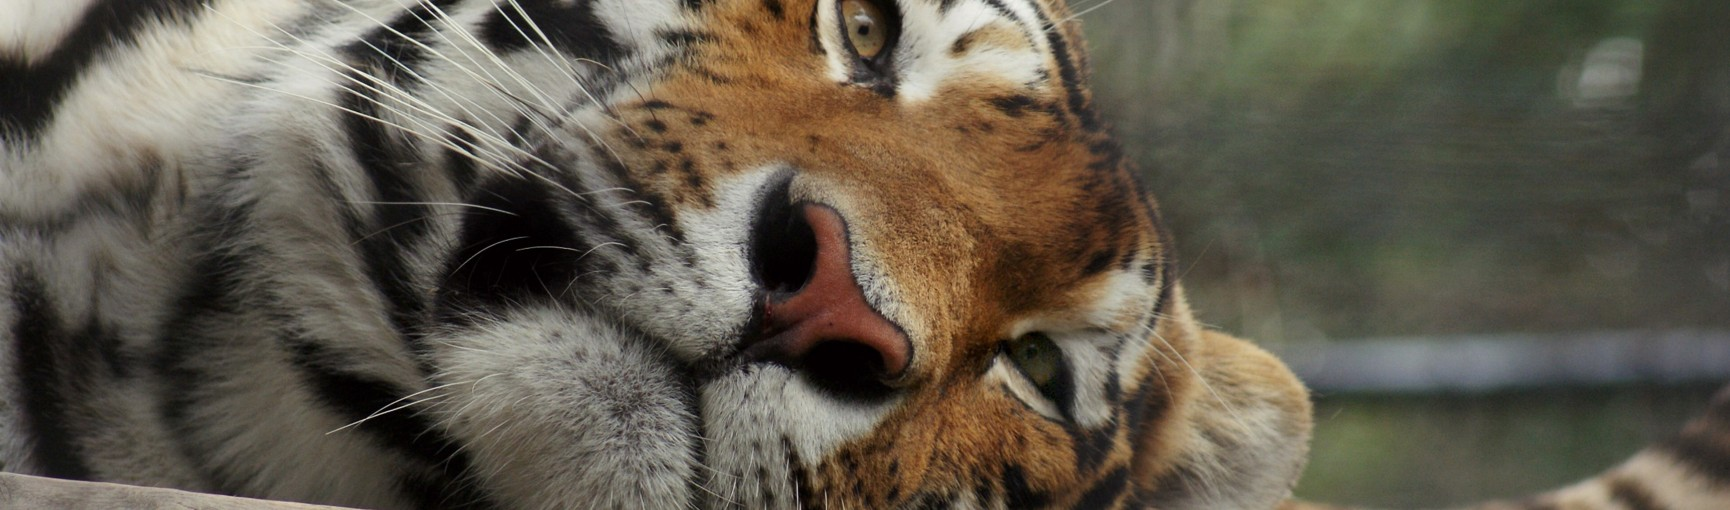
\includegraphics{animals/animal1.jpeg}
    \caption{Animal 1}
    \label{fig:animal1}
\end{figure}
\end{verbatim}
\end{scriptsize}
\begin{figure}
    \centering
    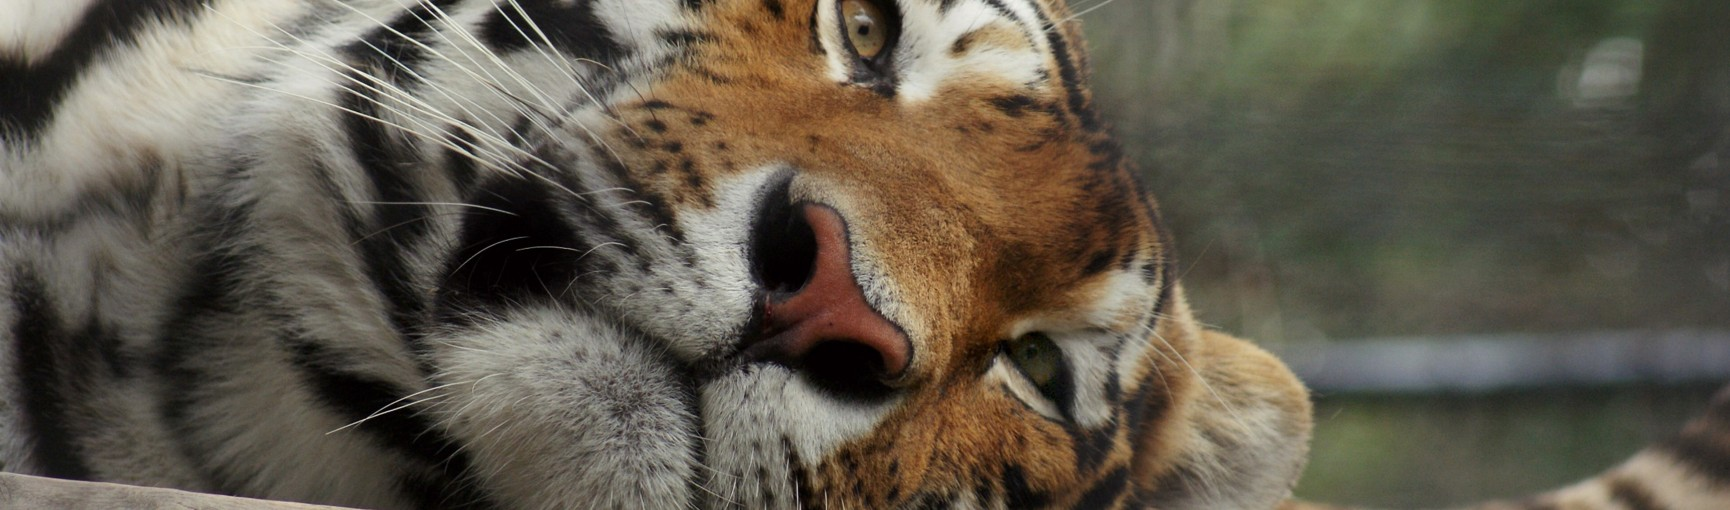
\includegraphics{animals/animal1.jpeg}
    \caption{Animal 1}
    \label{fig:animal1}
\end{figure}
\end{frame}
\begin{frame}[fragile]{Escalar imágenes.}
\begin{scriptsize}
\begin{verbatim}
\begin{figure}
    \centering
    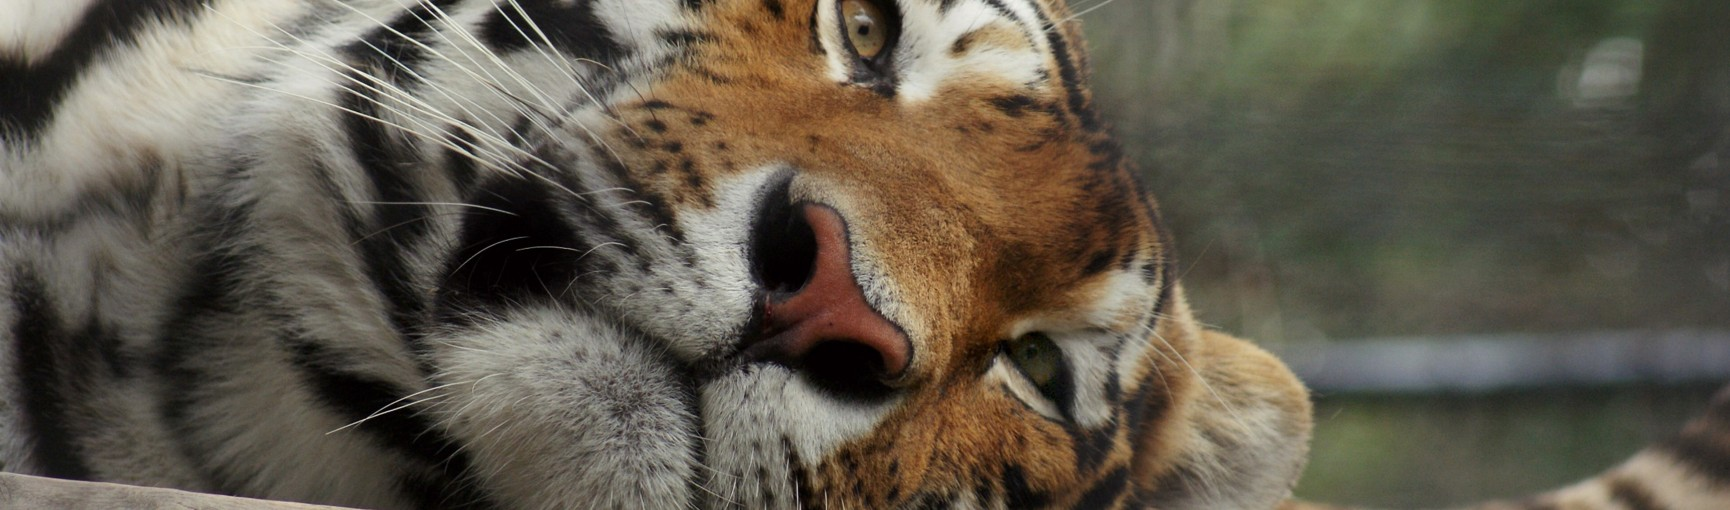
\includegraphics[scale=0.15]{animals/animal1.jpeg}
    \caption{Animal 1}
    \label{fig:animal1}
\end{figure}
\end{verbatim}
\end{scriptsize}
\begin{figure}
    \centering
    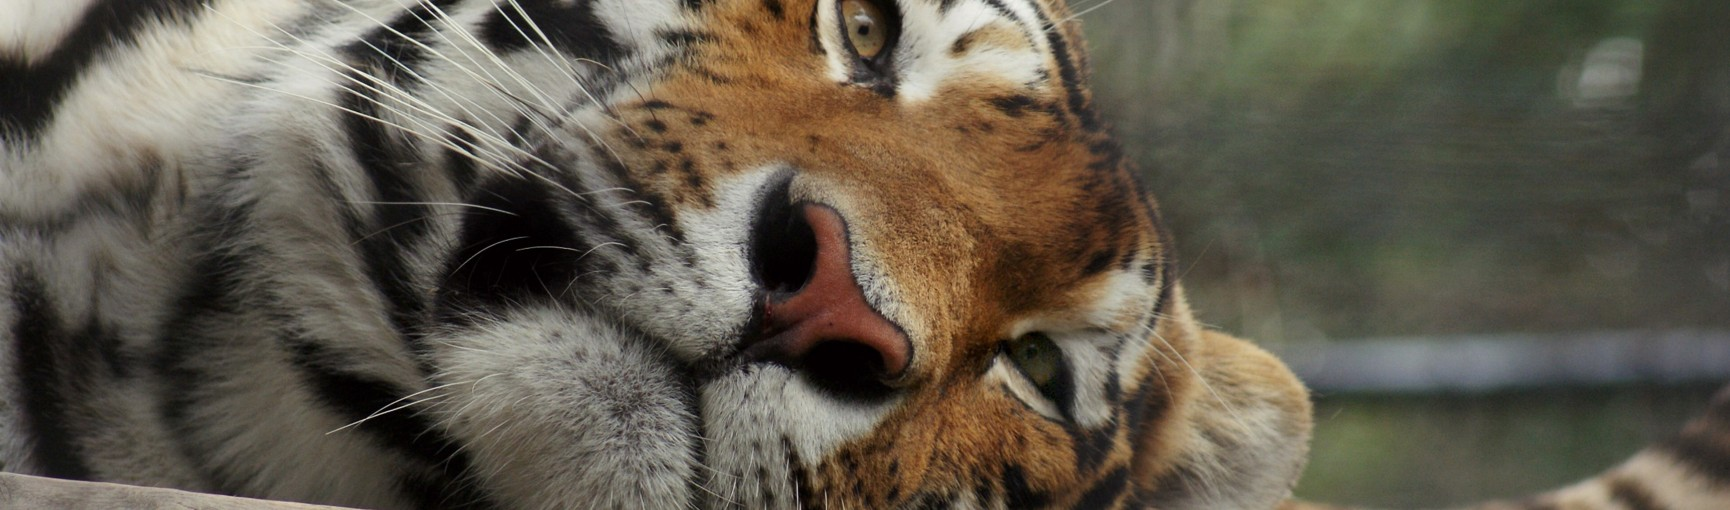
\includegraphics[scale=0.15]{animals/animal1.jpeg}
    \caption{Animal 1}
    \label{fig:animal1}
\end{figure}
\end{frame}

\subsection*{Ancho}
\begin{frame}[fragile]{Ancho de imágenes.}
\begin{scriptsize}
\begin{verbatim}
\begin{figure}
    \centering
    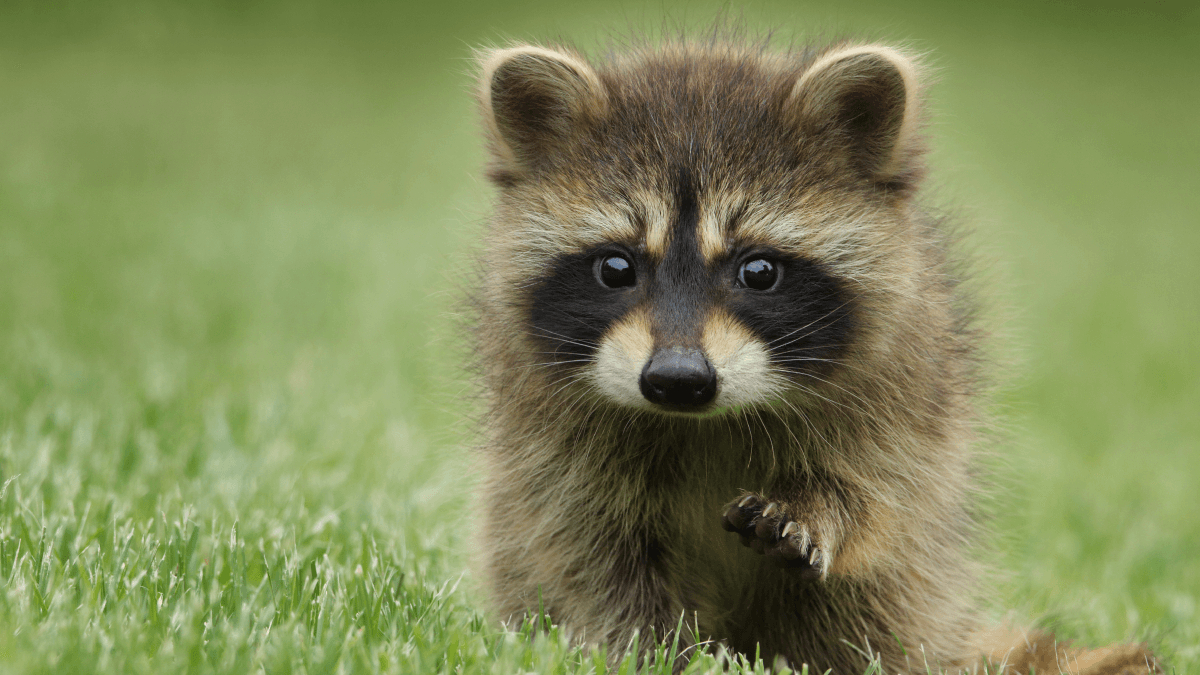
\includegraphics{animals/animal2.png}
    \caption{Animal 2}
\end{figure}
\end{verbatim}
\end{scriptsize}
\begin{figure}
    \centering
    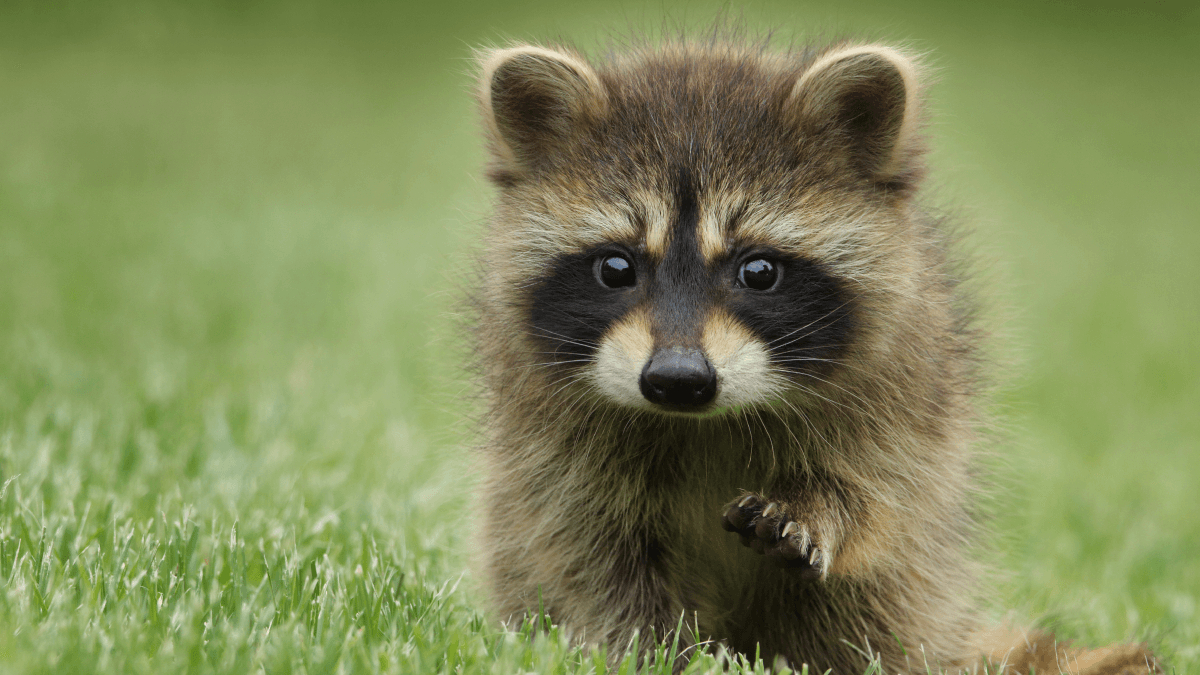
\includegraphics{animals/animal2.png}
    \caption{Animal 2}
\end{figure}
\end{frame}
\begin{frame}[fragile]{Ancho de imágenes.}
\begin{scriptsize}
\begin{verbatim}
\begin{figure}
    \centering
    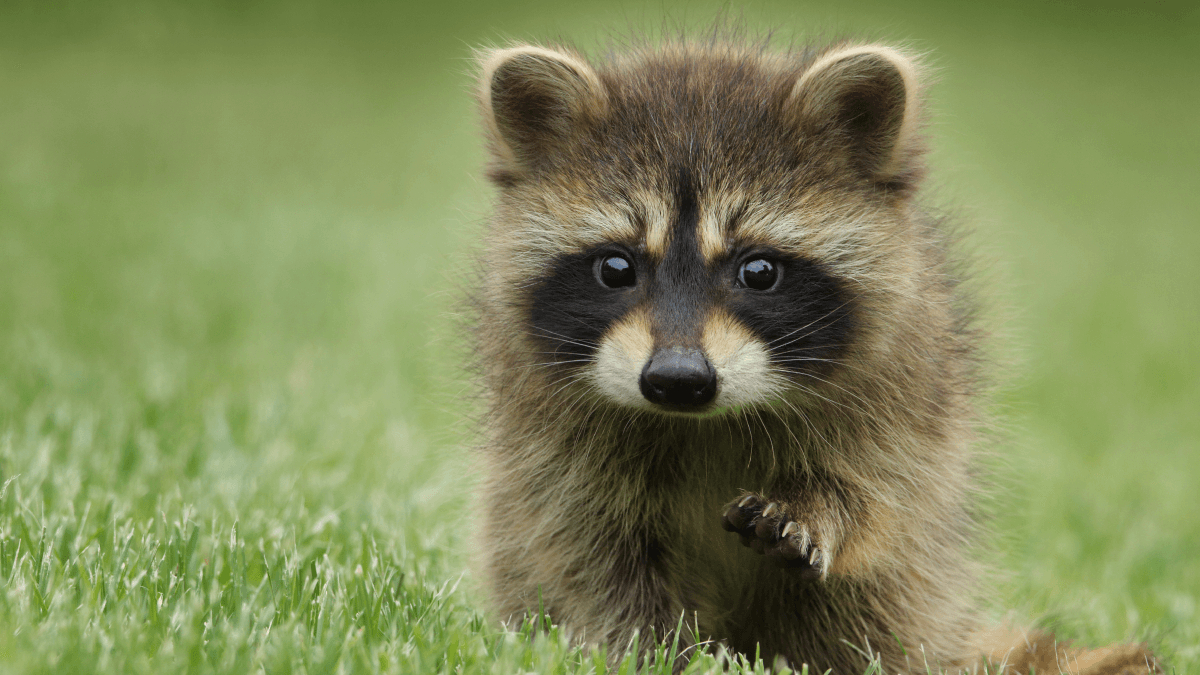
\includegraphics[width=10cm]{animals/animal2.png}
    \caption{Animal 2}
\end{figure}
\end{verbatim}
\end{scriptsize}
\begin{figure}
    \centering
    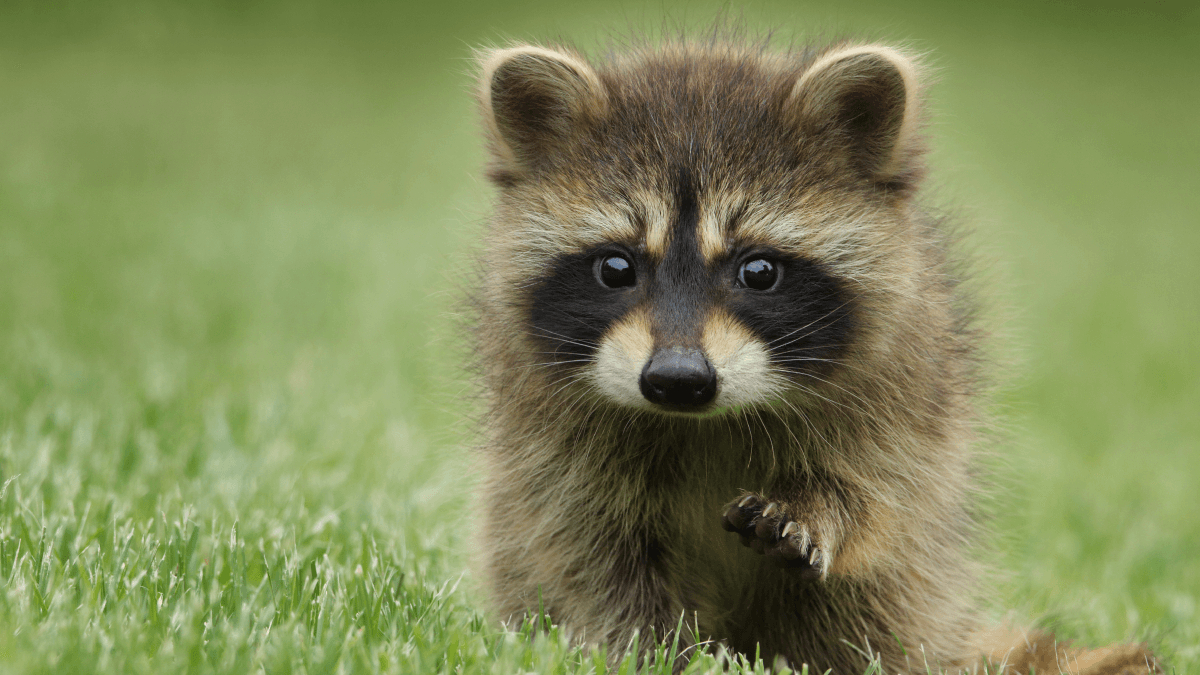
\includegraphics[width=10cm]{animals/animal2.png}
    \caption{Animal 2}
\end{figure}
\end{frame}
\begin{frame}[fragile]{Ancho de imágenes.}
\begin{scriptsize}
\begin{verbatim}
\begin{figure}
    \centering
    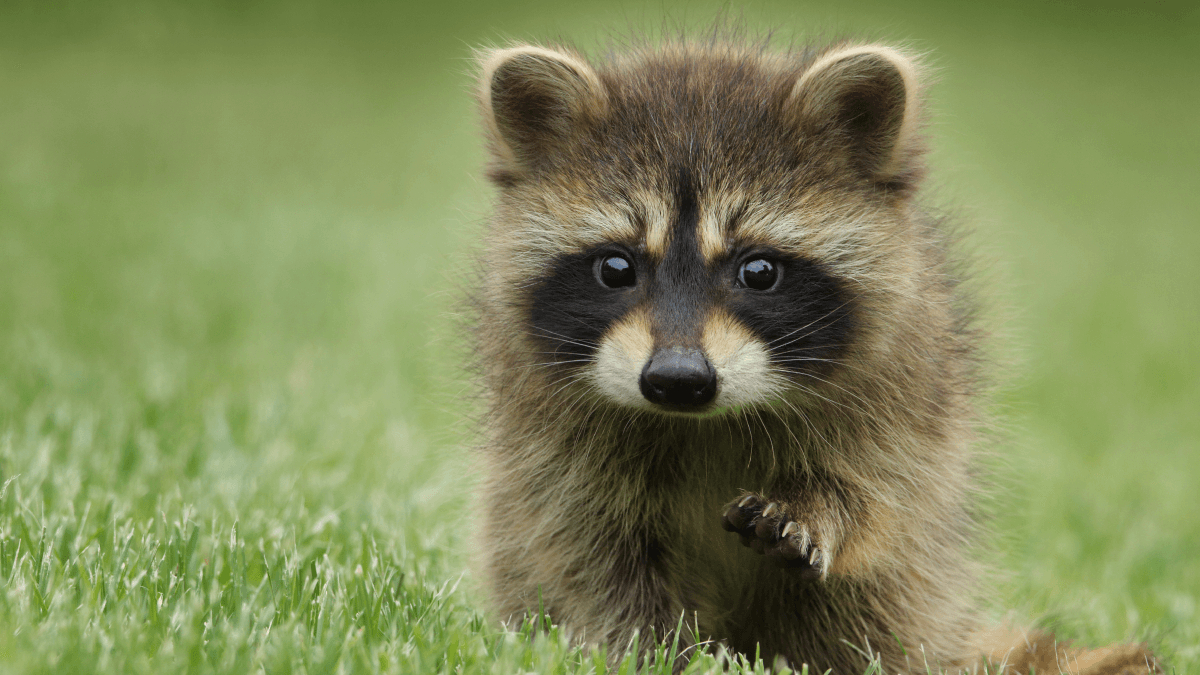
\includegraphics[width=0.5\linewidth]{animals/animal2.png}
    \caption{Animal 2}
\end{figure}
\end{verbatim}
\end{scriptsize}
\begin{figure}
    \centering
    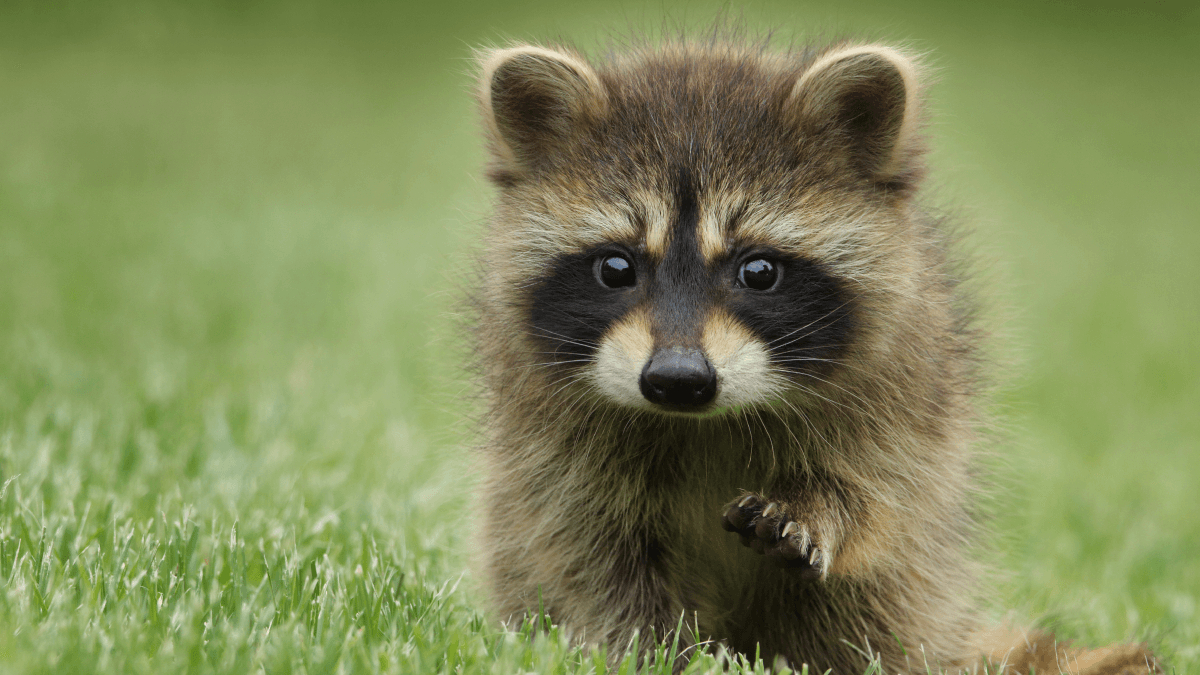
\includegraphics[width=0.5\linewidth]{animals/animal2.png}
    \caption{Animal 2}
\end{figure}
\end{frame}

\subsection*{Alto}
\begin{frame}[fragile]{Alto de imágenes.}
\begin{scriptsize}
\begin{verbatim}
\begin{figure}
    \centering
    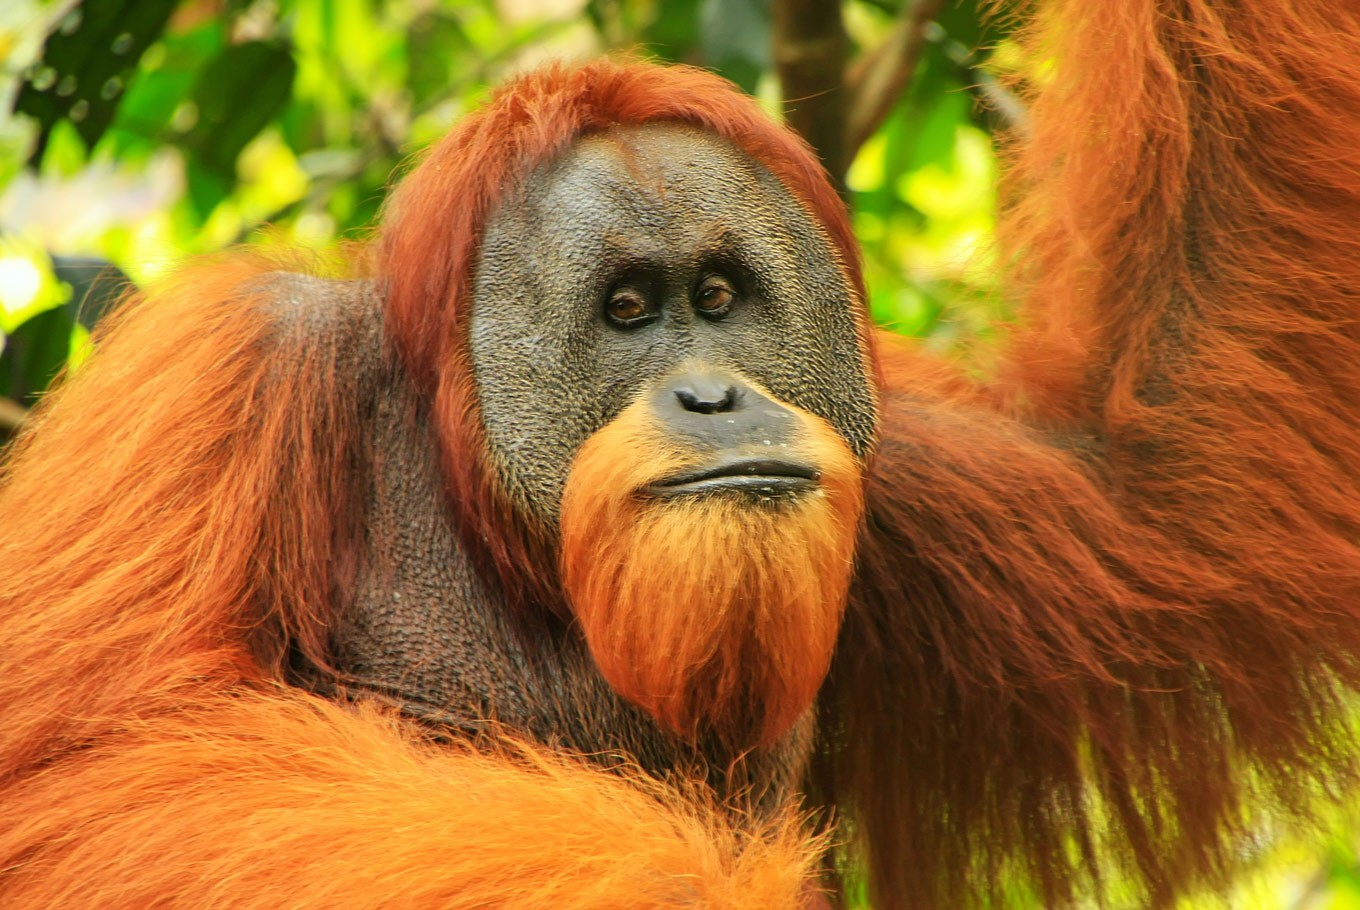
\includegraphics{animals/animal3.jpg}
    \caption{Animal 3}
\end{figure}
\end{verbatim}
\end{scriptsize}
\begin{figure}
    \centering
    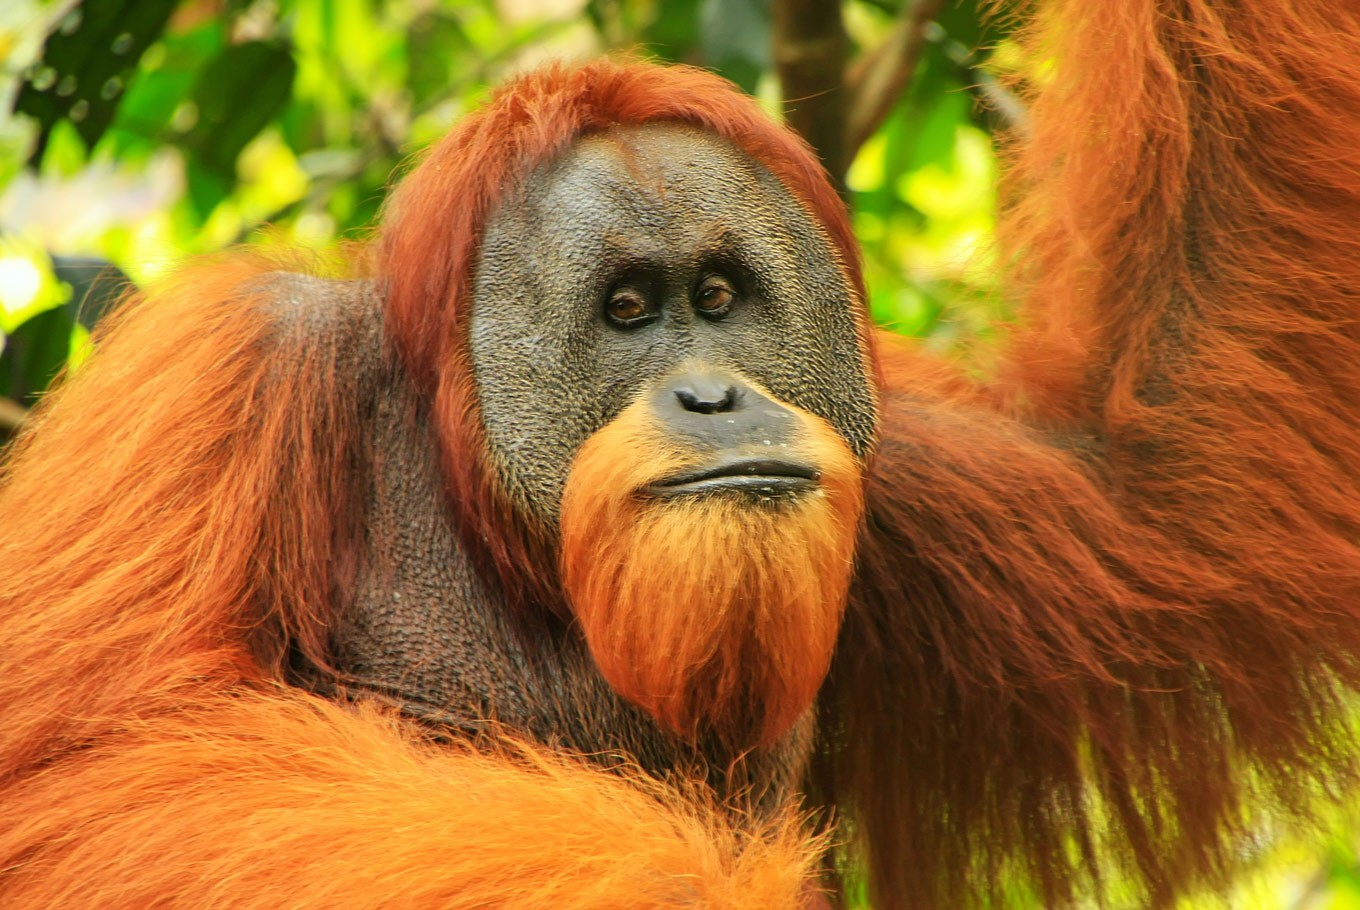
\includegraphics{animals/animal3.jpg}
    \caption{Animal 3}
\end{figure}
\end{frame}
\begin{frame}[fragile]{Alto de imágenes.}
\begin{scriptsize}
\begin{verbatim}
\begin{figure}
    \centering
    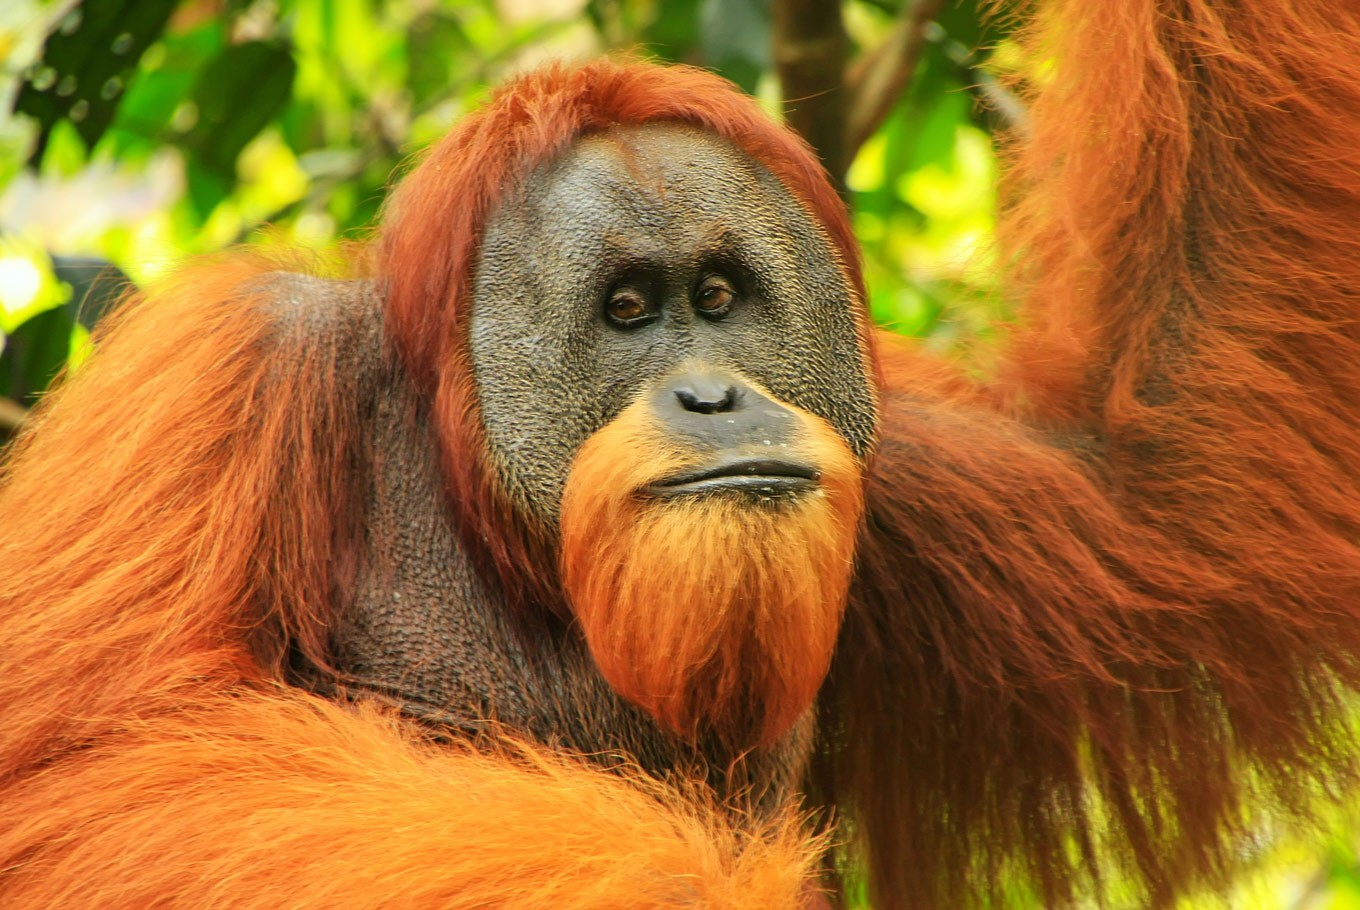
\includegraphics[height=4cm]{animals/animal3.jpg}
    \caption{Animal 3}
\end{figure}
\end{verbatim}
\end{scriptsize}
\begin{figure}
    \centering
    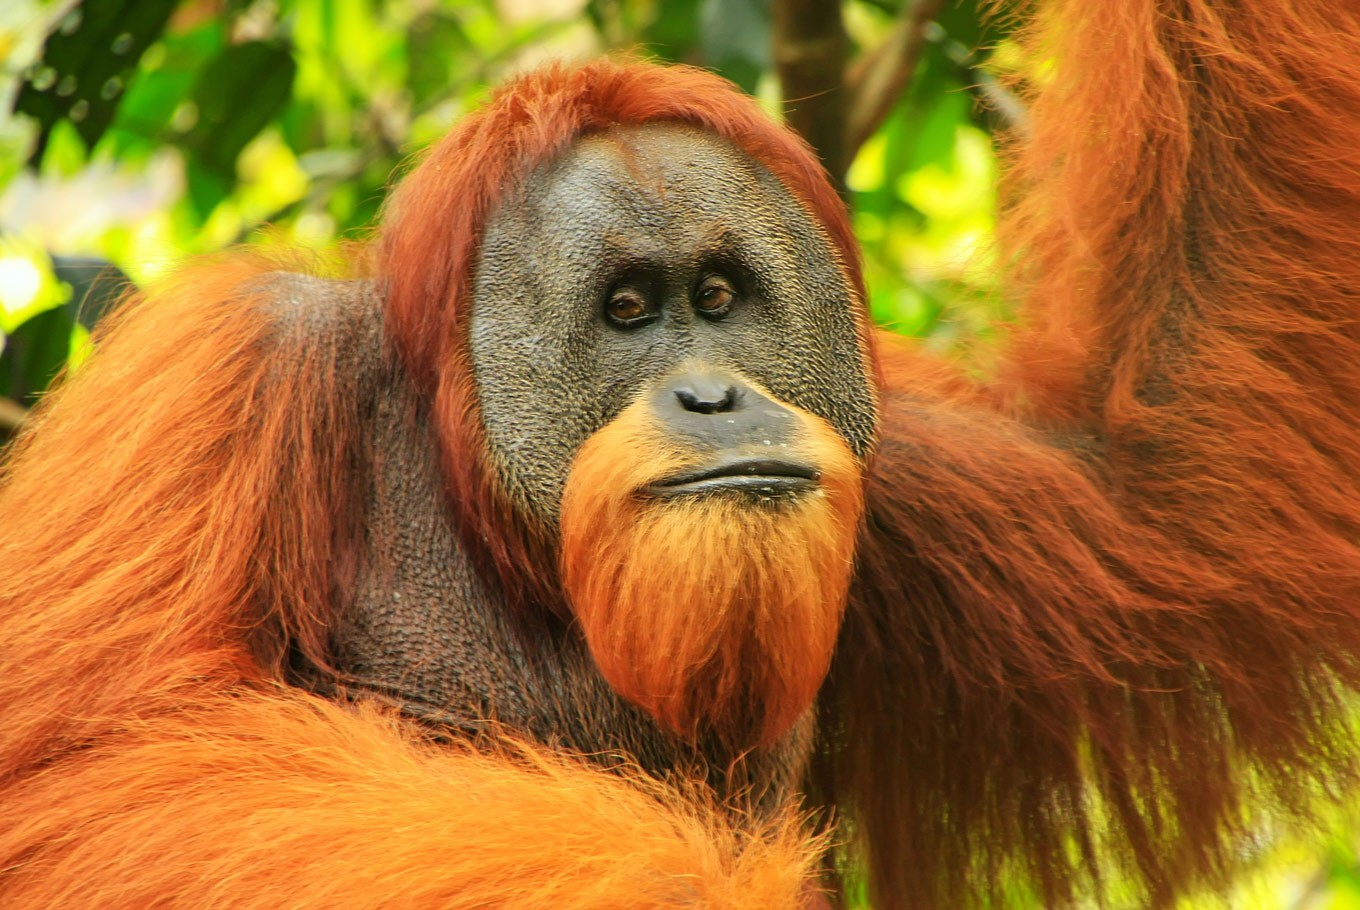
\includegraphics[height=4cm]{animals/animal3.jpg}
    \caption{Animal 3}
\end{figure}
\end{frame}

\subsection*{Ancho y alto}
\begin{frame}[fragile]{Ancho y alto de imágenes.}
\begin{scriptsize}
\begin{verbatim}
\begin{figure}
    \centering
    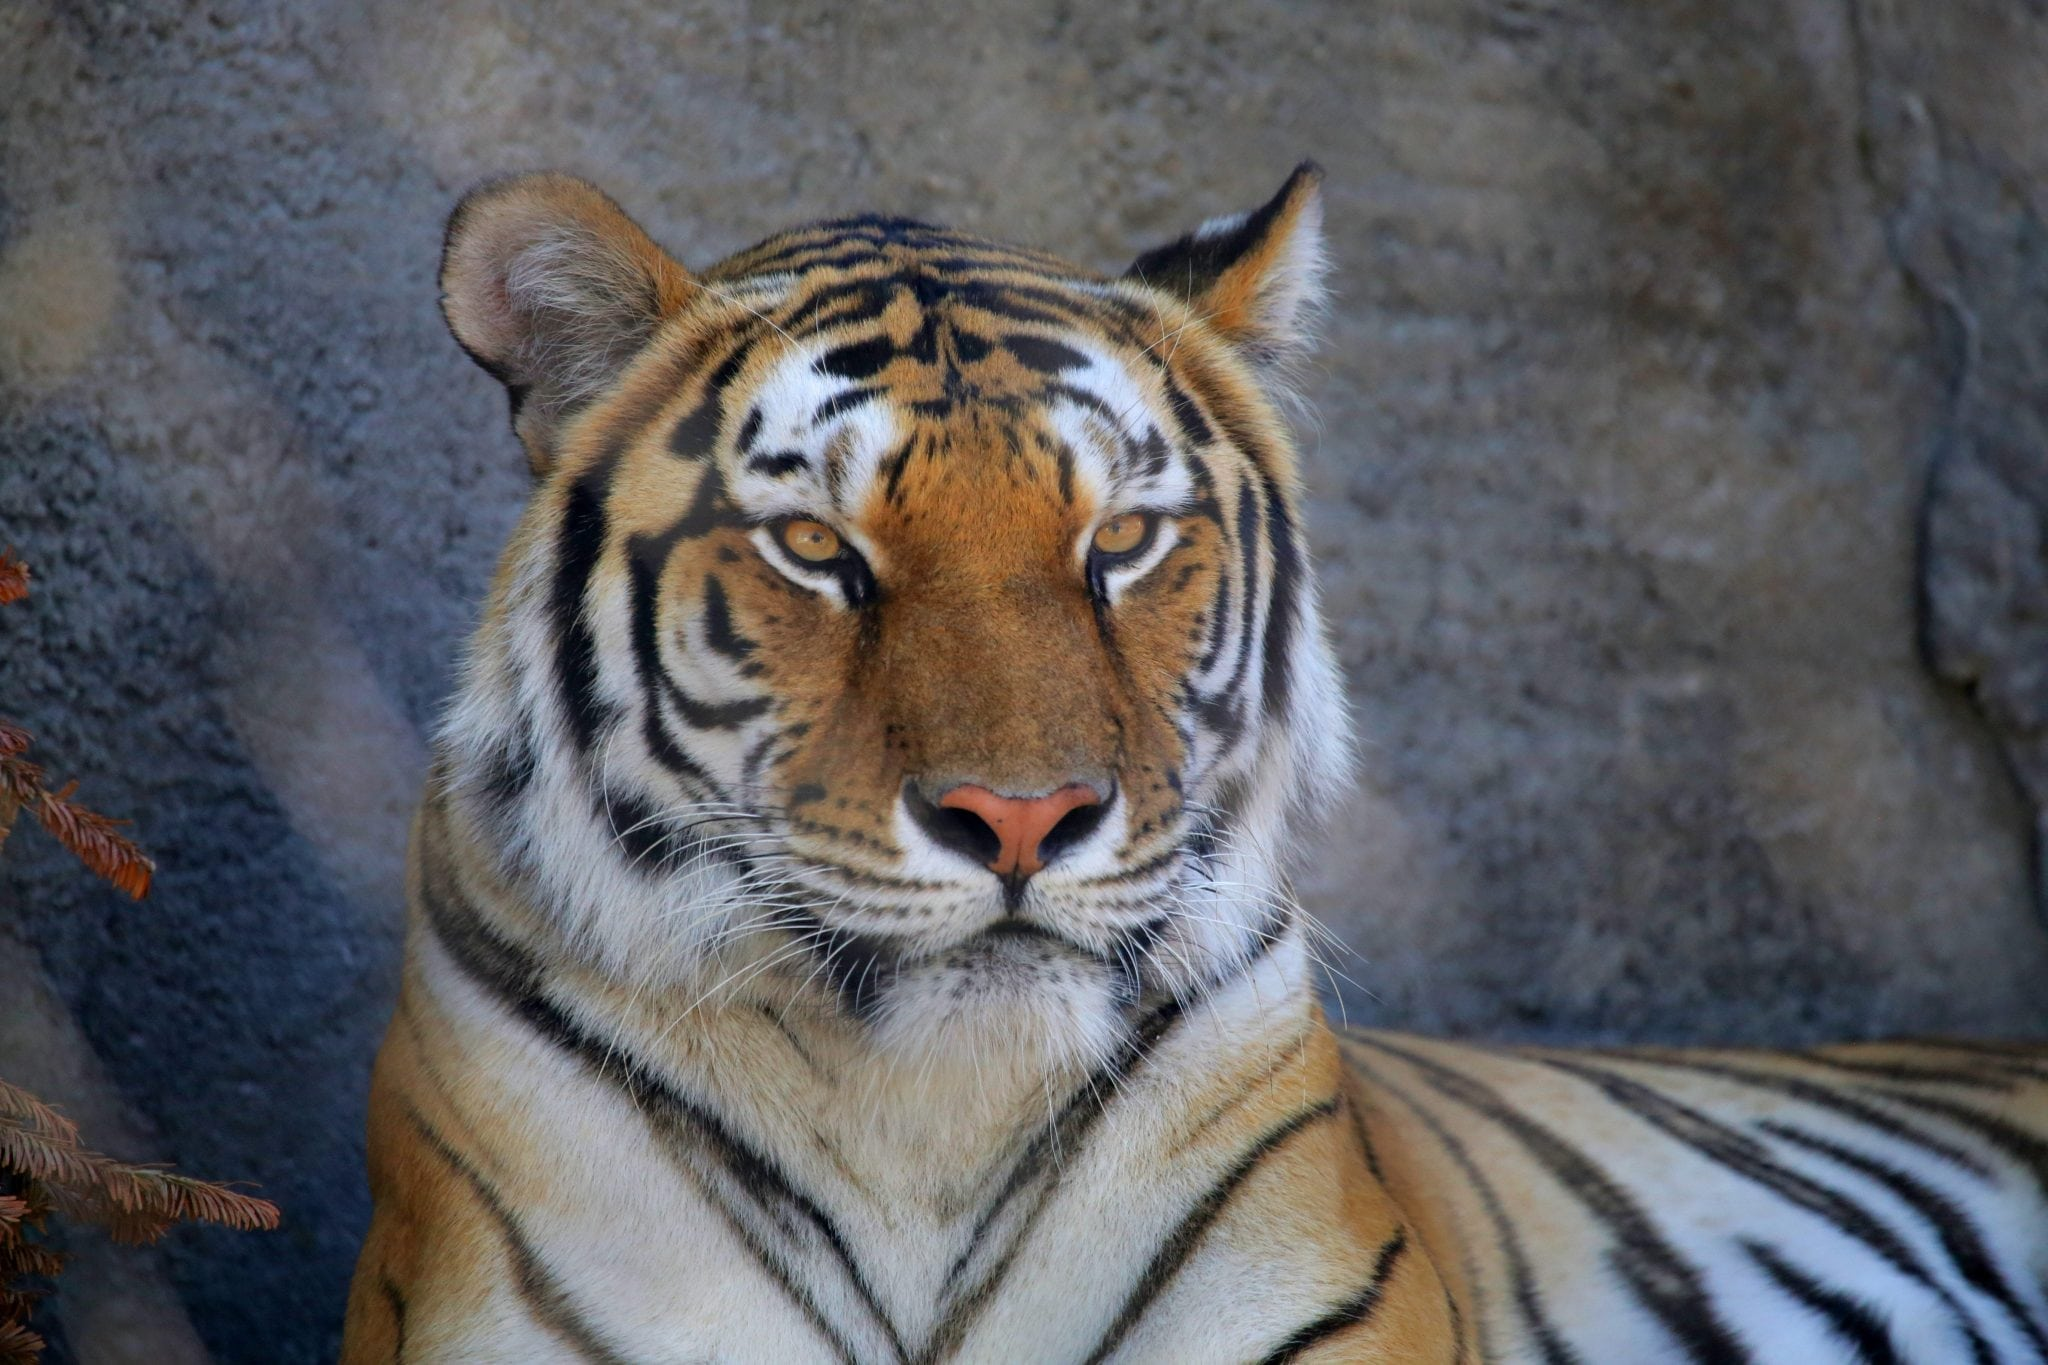
\includegraphics{animals/animal4.jpg}
    \caption{Animal 4}
\end{figure}
\end{verbatim}
\end{scriptsize}
\begin{figure}
    \centering
    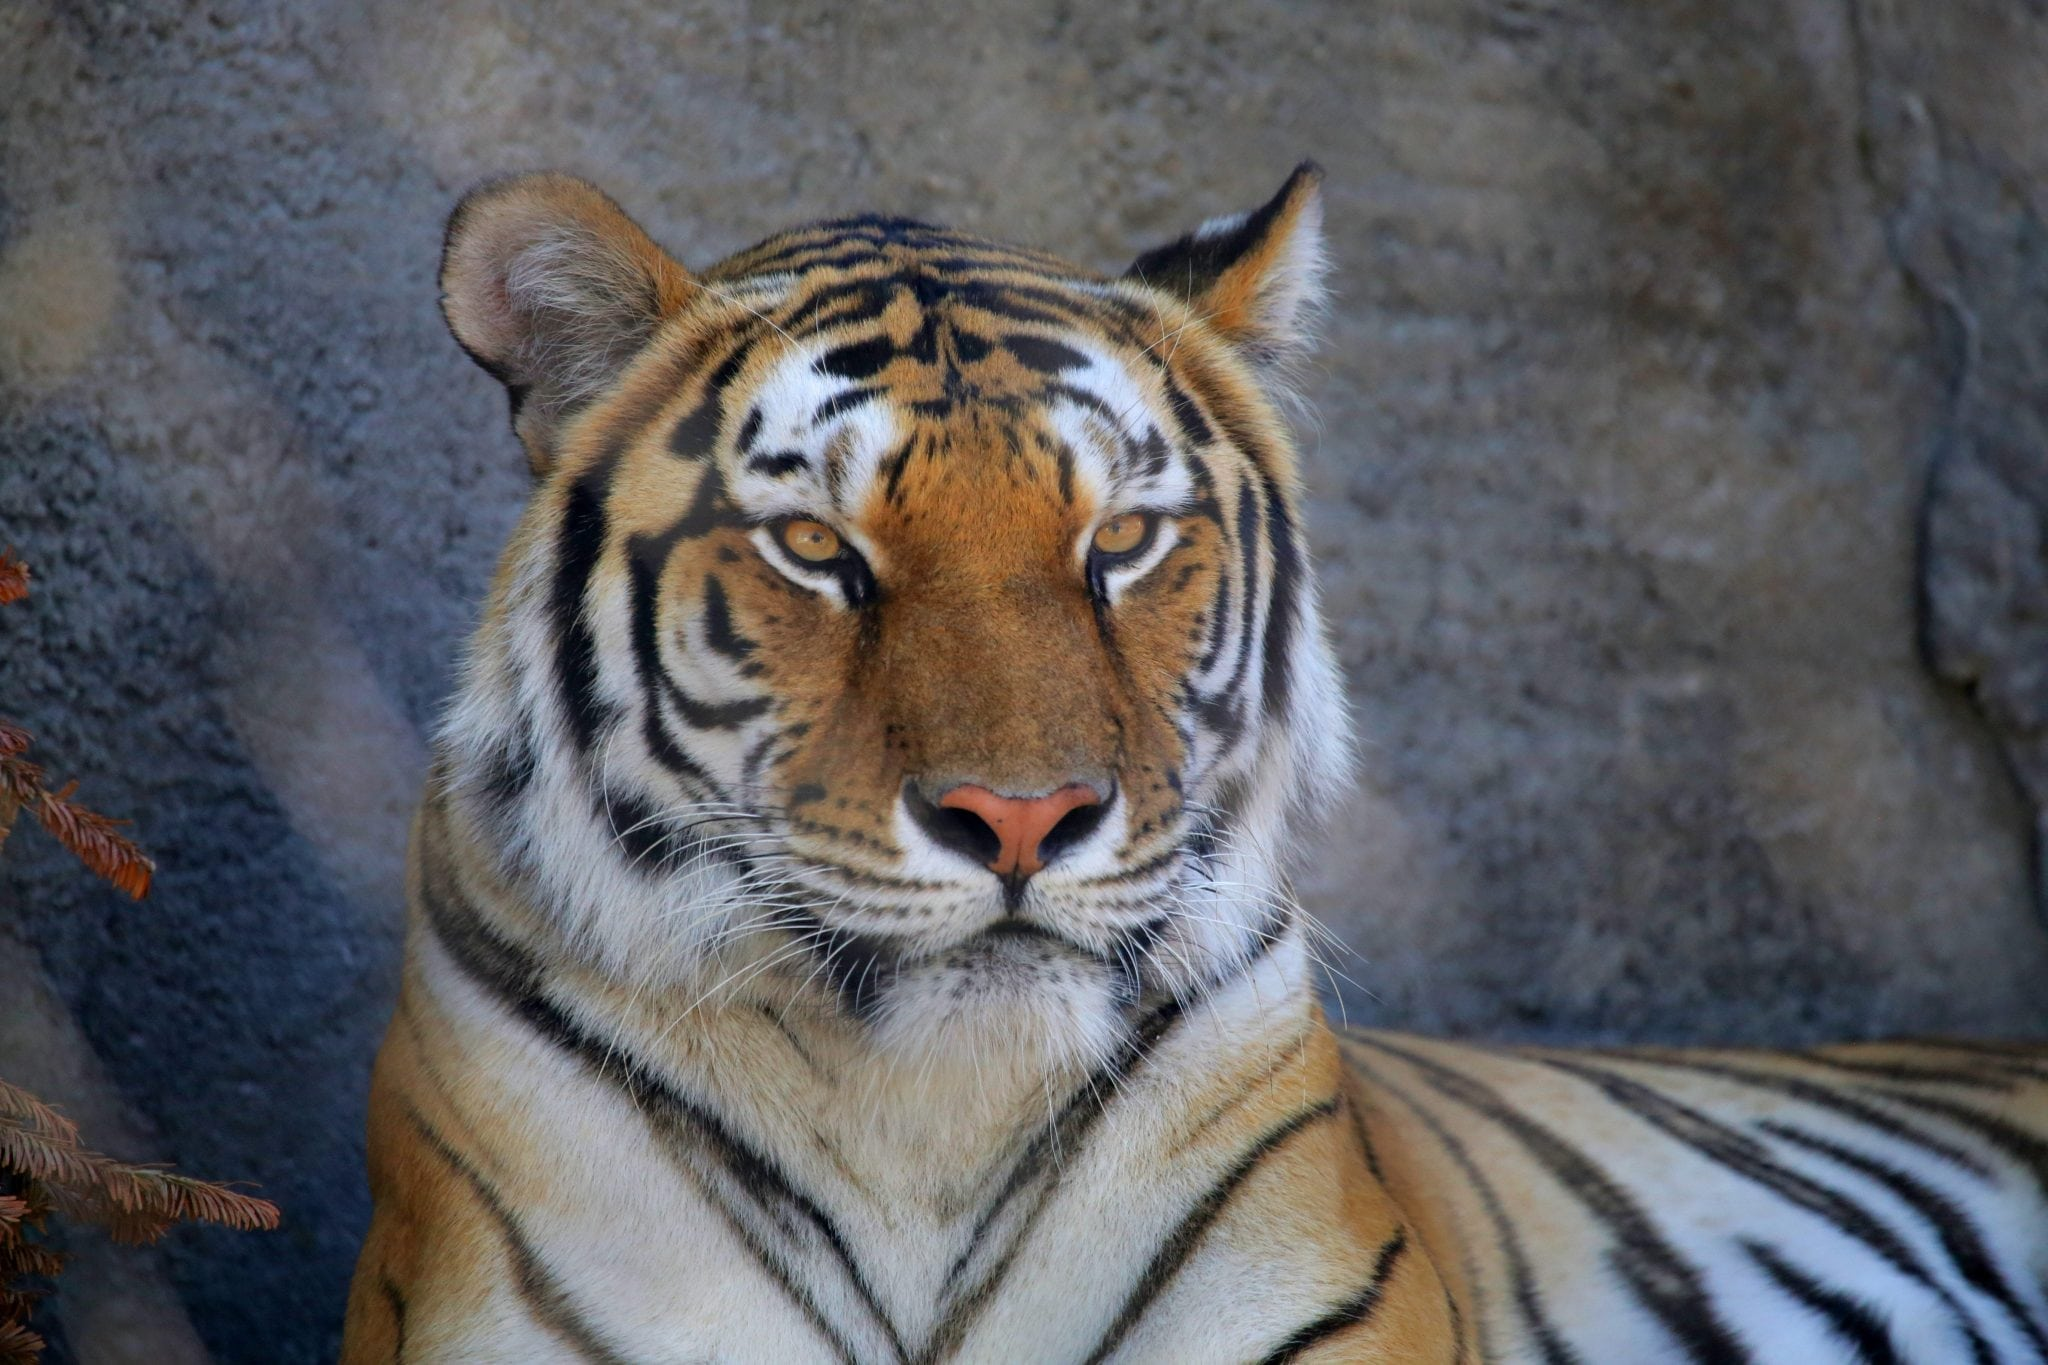
\includegraphics{animals/animal4.jpg}
    \caption{Animal 4}
\end{figure}
\end{frame}
\begin{frame}[fragile]{Ancho y alto de imágenes.}
\begin{scriptsize}
\begin{verbatim}
\begin{figure}
    \centering
    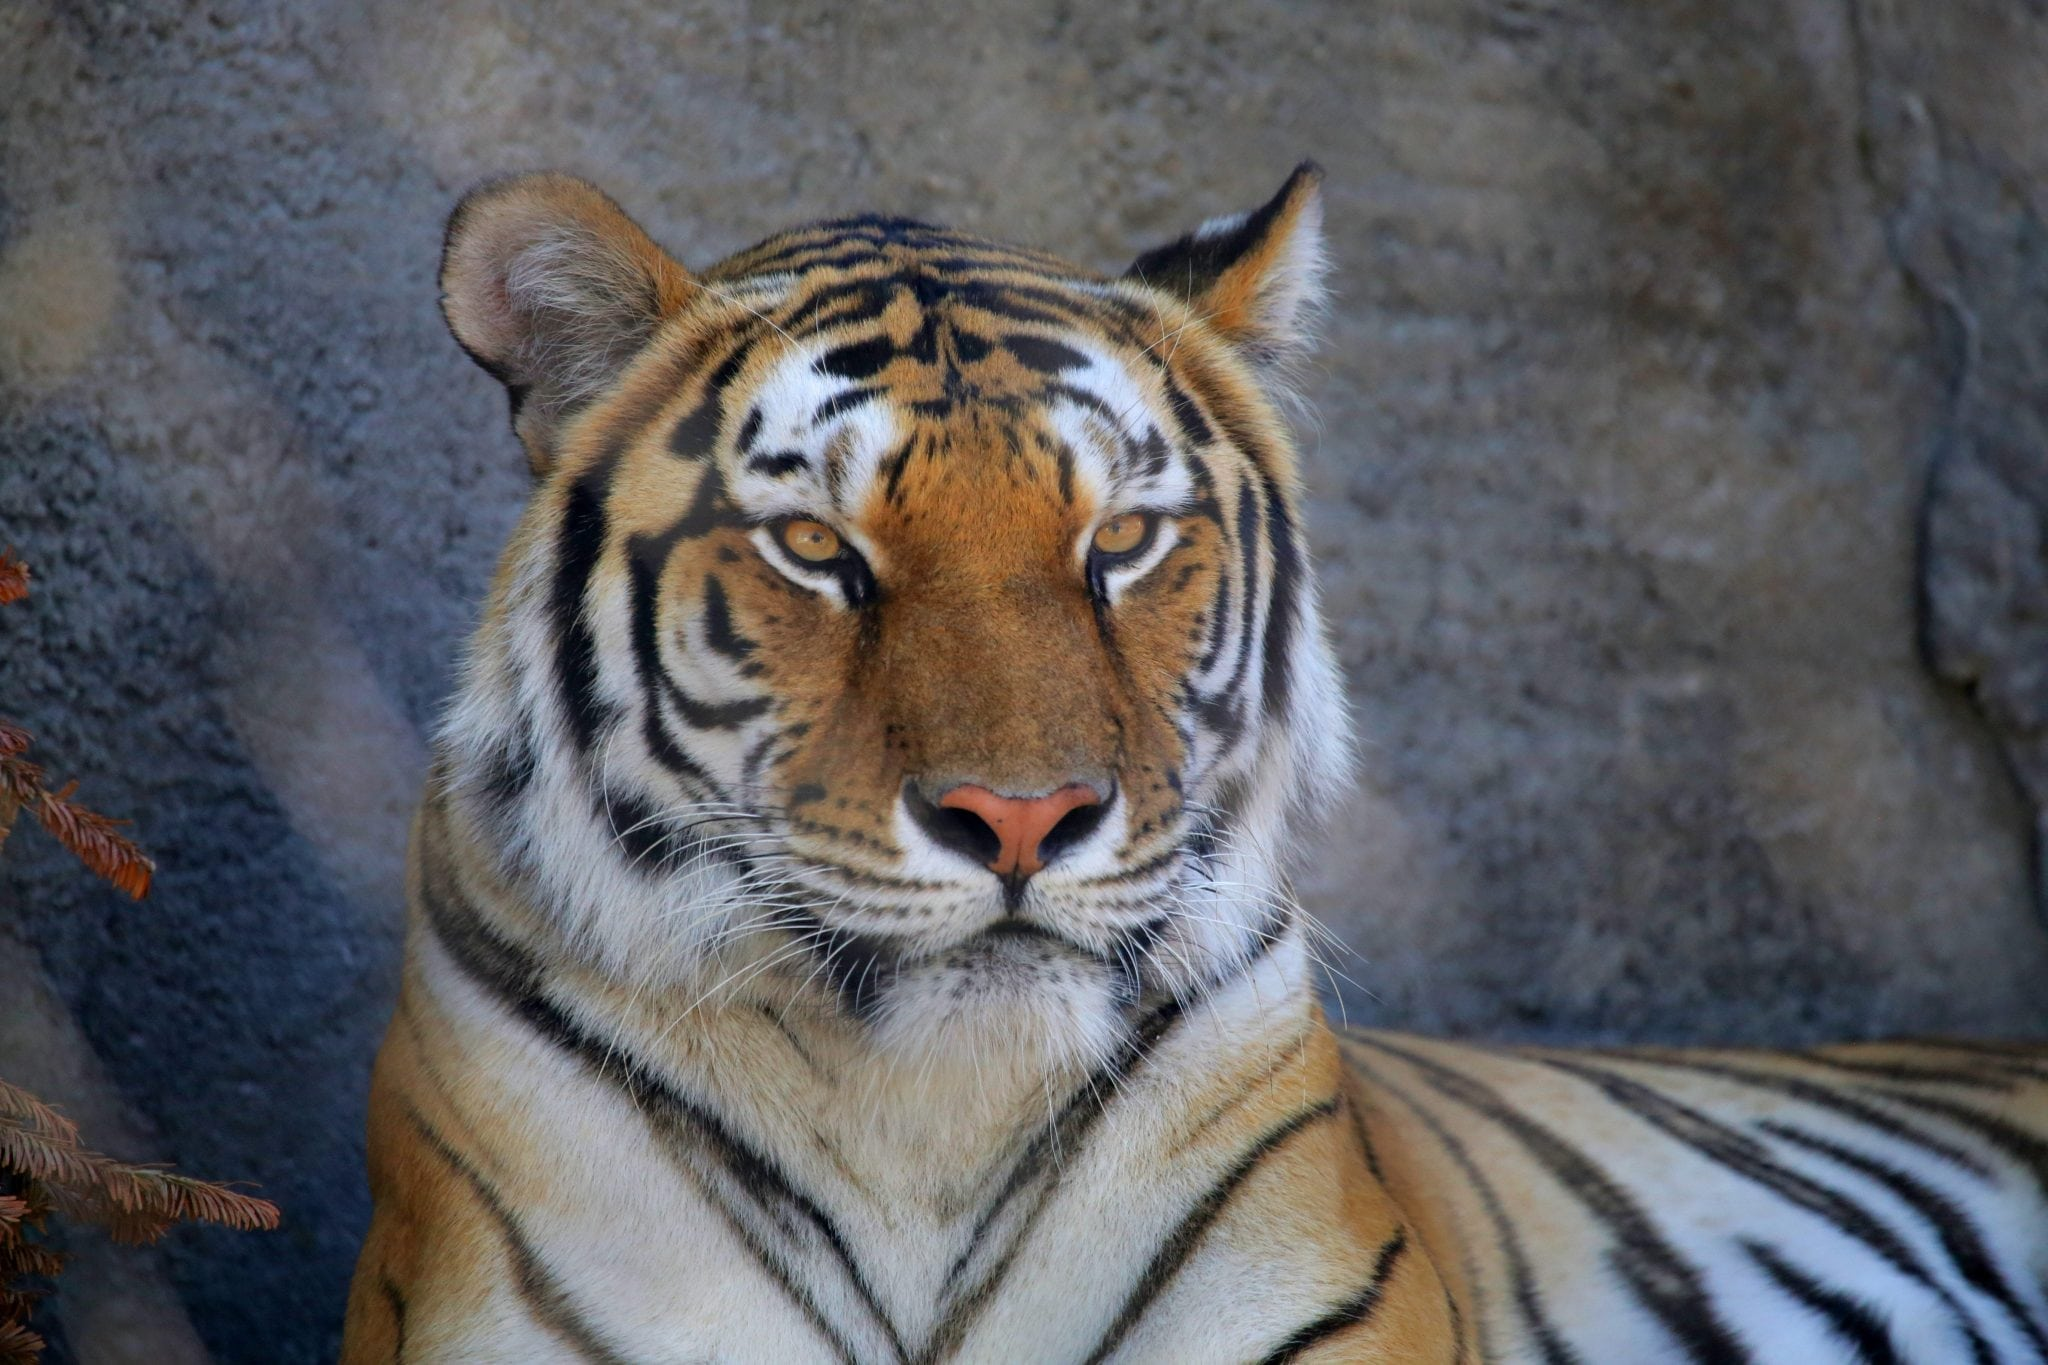
\includegraphics[width=2cm , height=4cm]{animals/animal4.jpg}
    \caption{Animal 4}
\end{figure}
\end{verbatim}
\end{scriptsize}
\begin{figure}
    \centering
    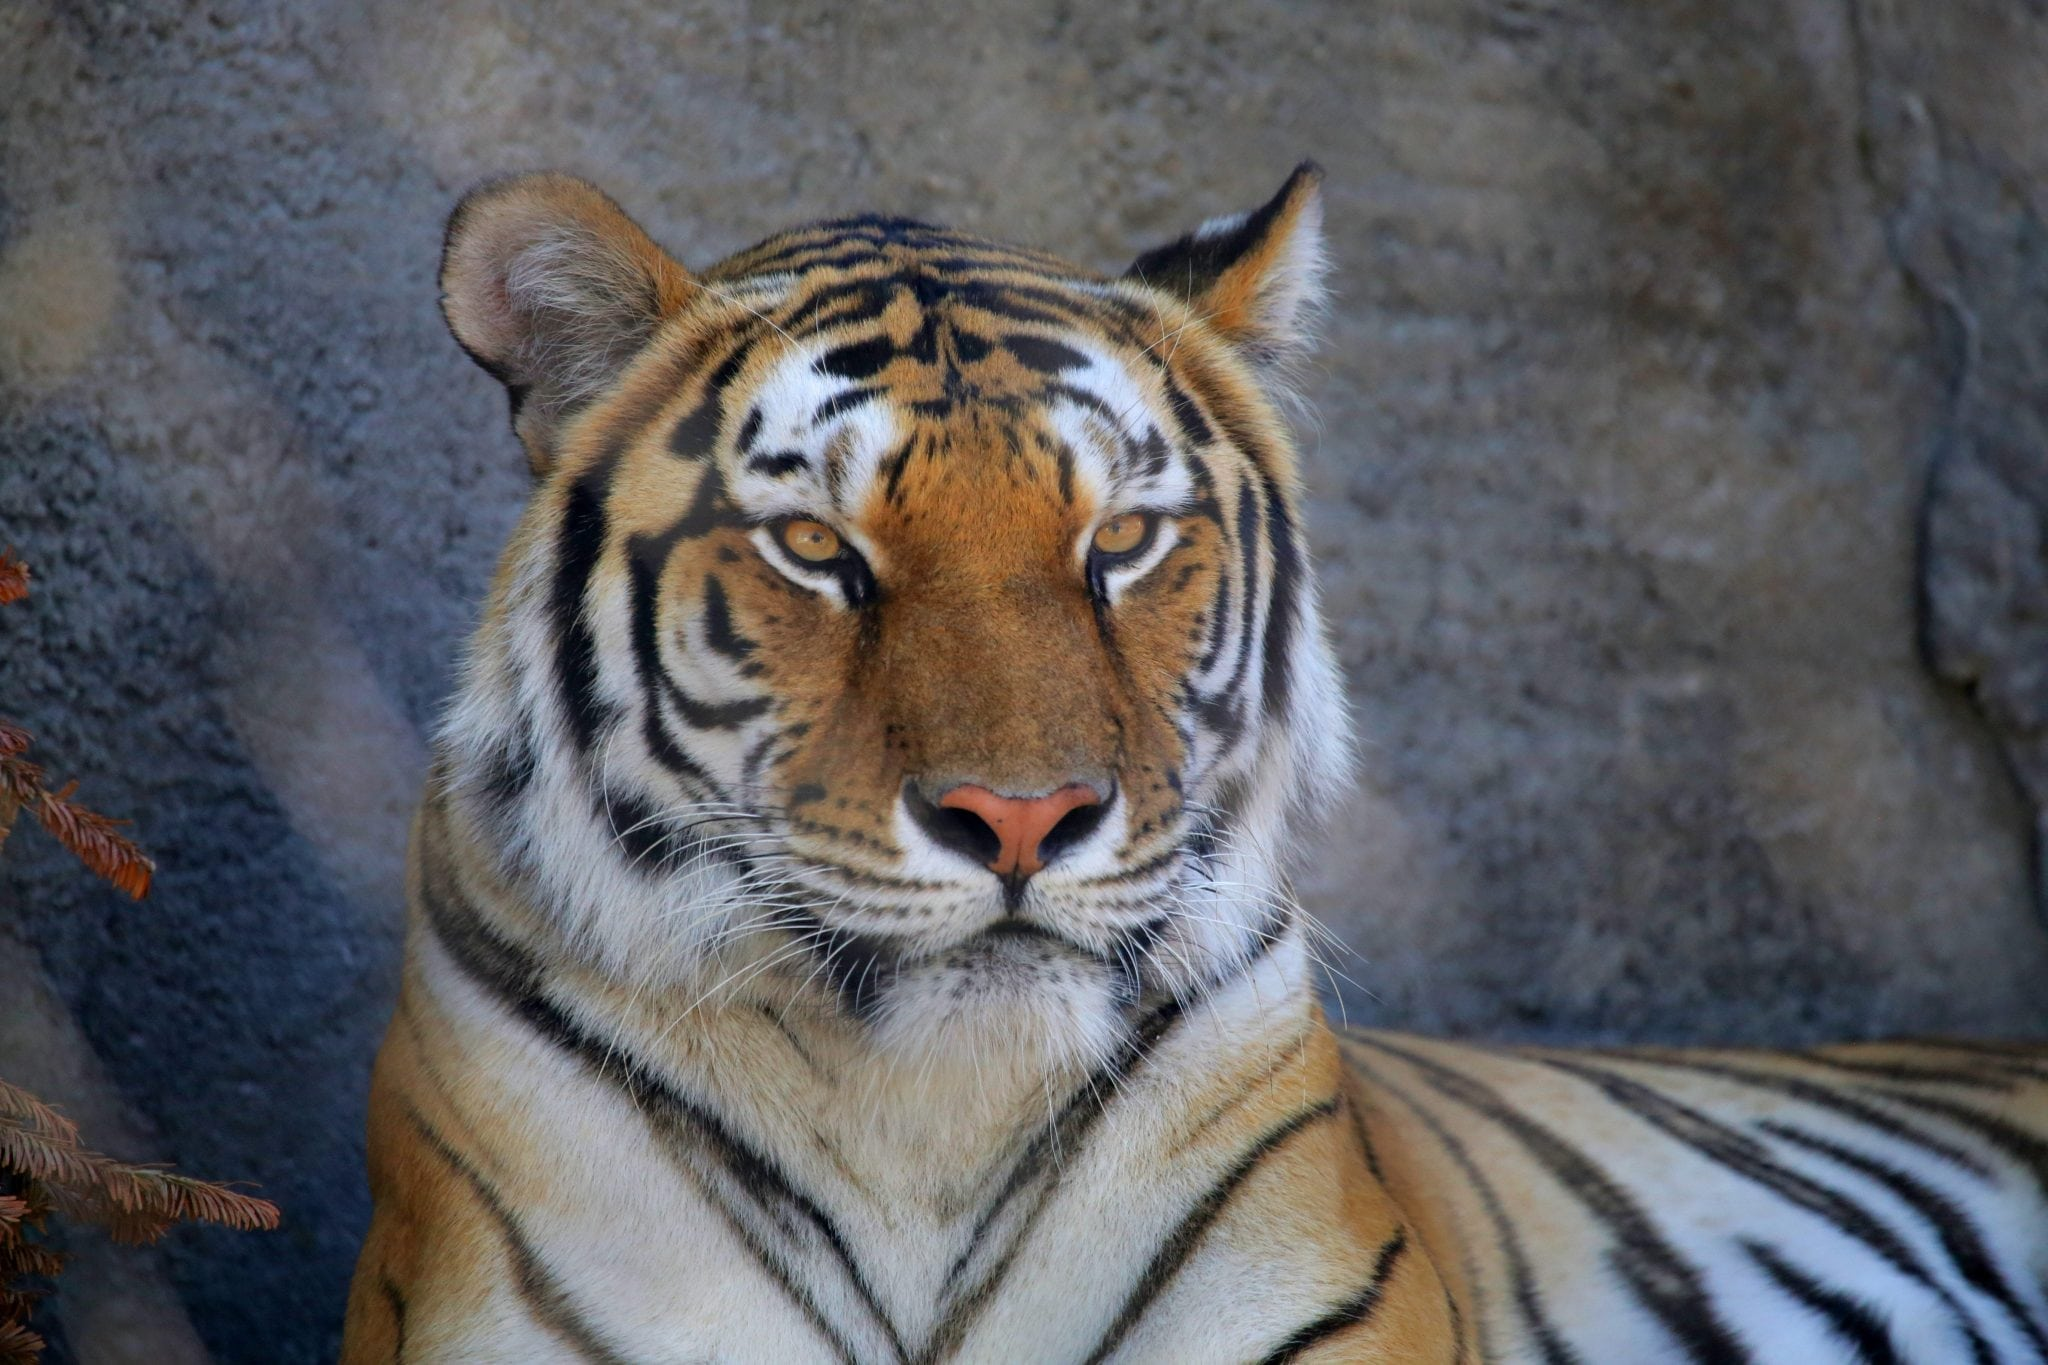
\includegraphics[width=8cm , height=3cm]{animals/animal4.jpg}
    \caption{Animal 4}
\end{figure}
\end{frame}

\subsection*{Rotar}
\begin{frame}[fragile]{Rotar.}
\begin{scriptsize}
\begin{verbatim}
\begin{figure}
    \centering
    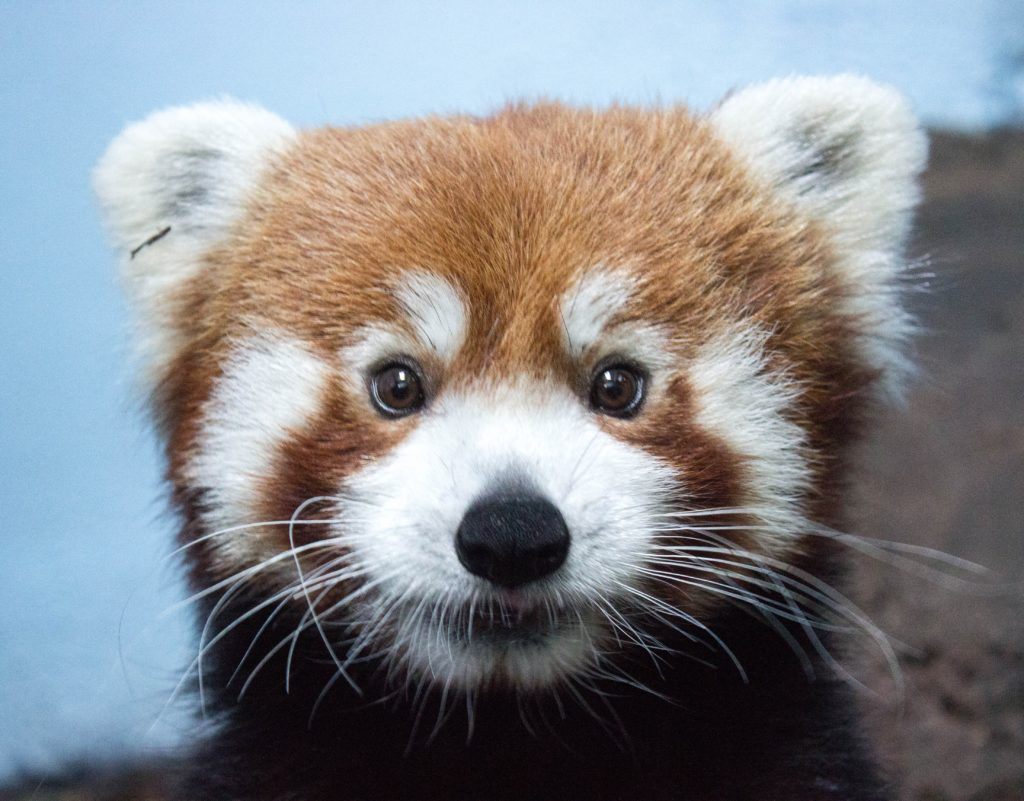
\includegraphics[width=0.4\linewidth]{animals/animal5.jpg}
    \caption{Animal 5}
\end{figure}
\end{verbatim}
\end{scriptsize}
\begin{figure}
    \centering
    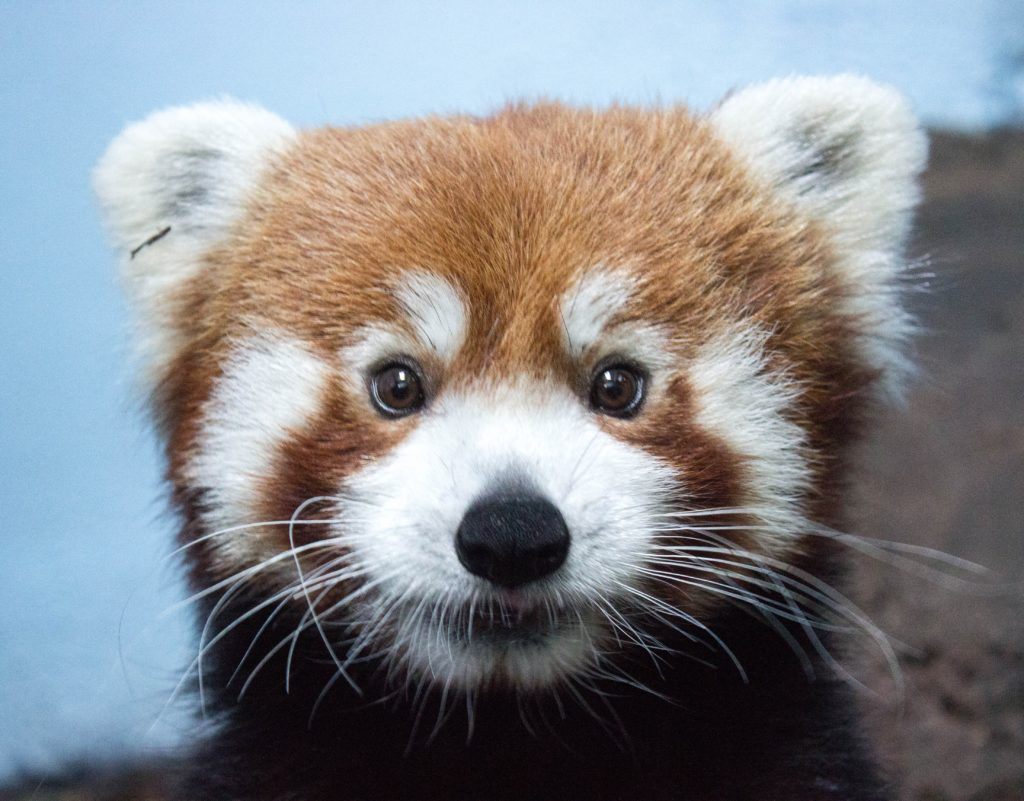
\includegraphics[width=0.4\linewidth]{animals/animal5.jpg}
    \caption{Animal 5}
\end{figure}
\end{frame}
\begin{frame}[fragile]{Rotar.}
\begin{scriptsize}
\begin{verbatim}
\begin{figure}
    \centering
    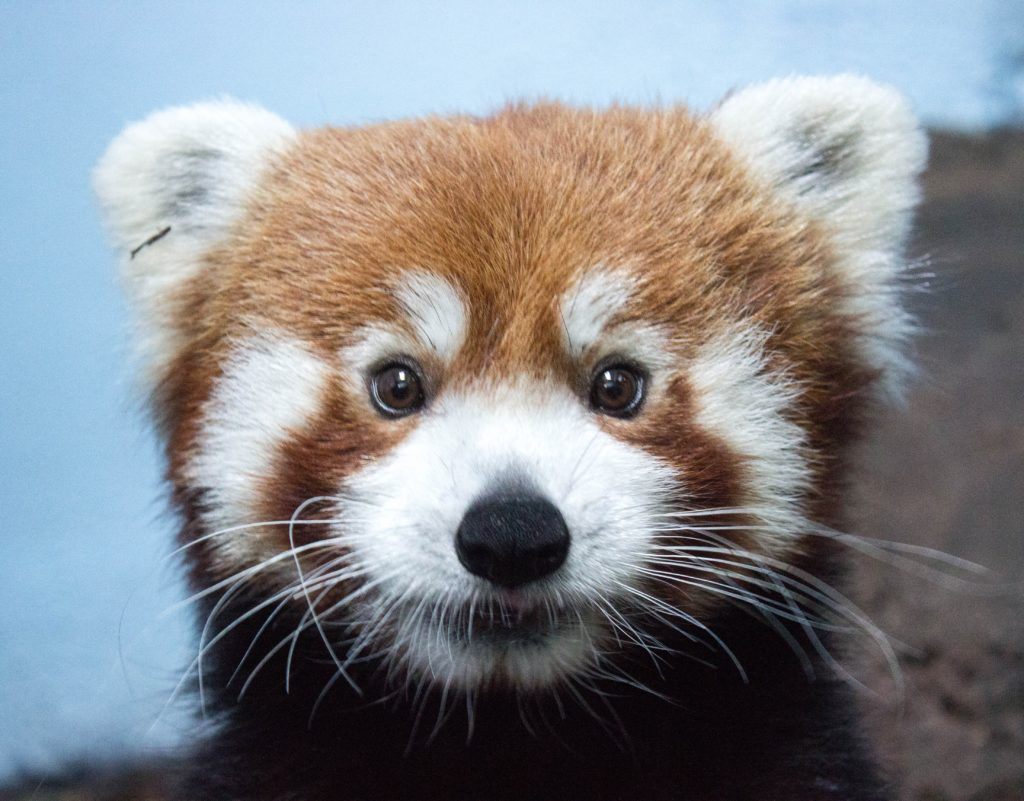
\includegraphics[width=0.4\linewidth, angle=45]{animals/animal5.jpg}
    \caption{Animal 5}
\end{figure}
\end{verbatim}
\end{scriptsize}
\vspace*{-1.5cm}
\begin{figure}
    \centering
    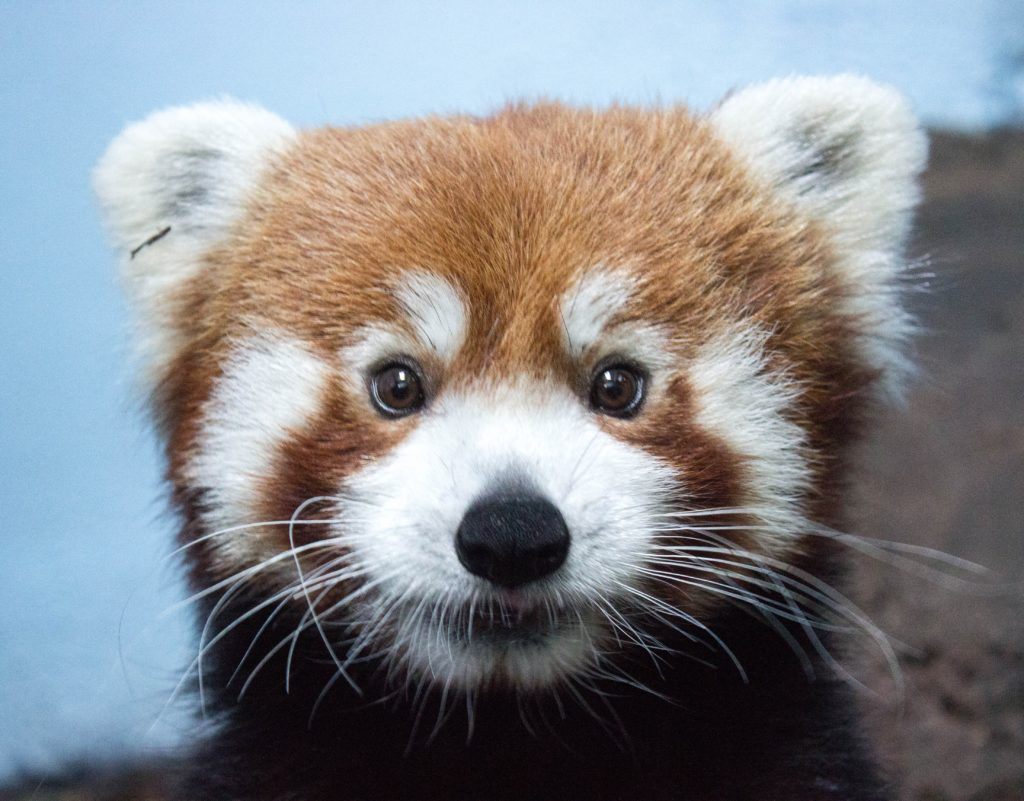
\includegraphics[width=0.4\linewidth, angle=45]{animals/animal5.jpg}
    \caption{Animal 5}
\end{figure}
\end{frame}

\section{Sub-imágenes.}
\begin{frame}{Contenido.}
  \tableofcontents[currentsection]
\end{frame}
\begin{frame}[fragile]{Sub-imágenes.}
    Para insertar varias imágenes como sub-imágenes hay dos formas:
    \begin{itemize}
        \item Usar minipages dentro de el ambiente \verb!figure!.
        \item Usar el paquete \verb!subcaption! (Hay que importarlo en el preámbulo).
    \end{itemize}
\end{frame}

\begin{frame}[fragile]{Sub-imágenes: \itshape minipages.}
\begin{scriptsize}
\begin{verbatim}
\begin{figure}
    \centering
    \begin{minipage}{0.4\linewidth}
    \centering 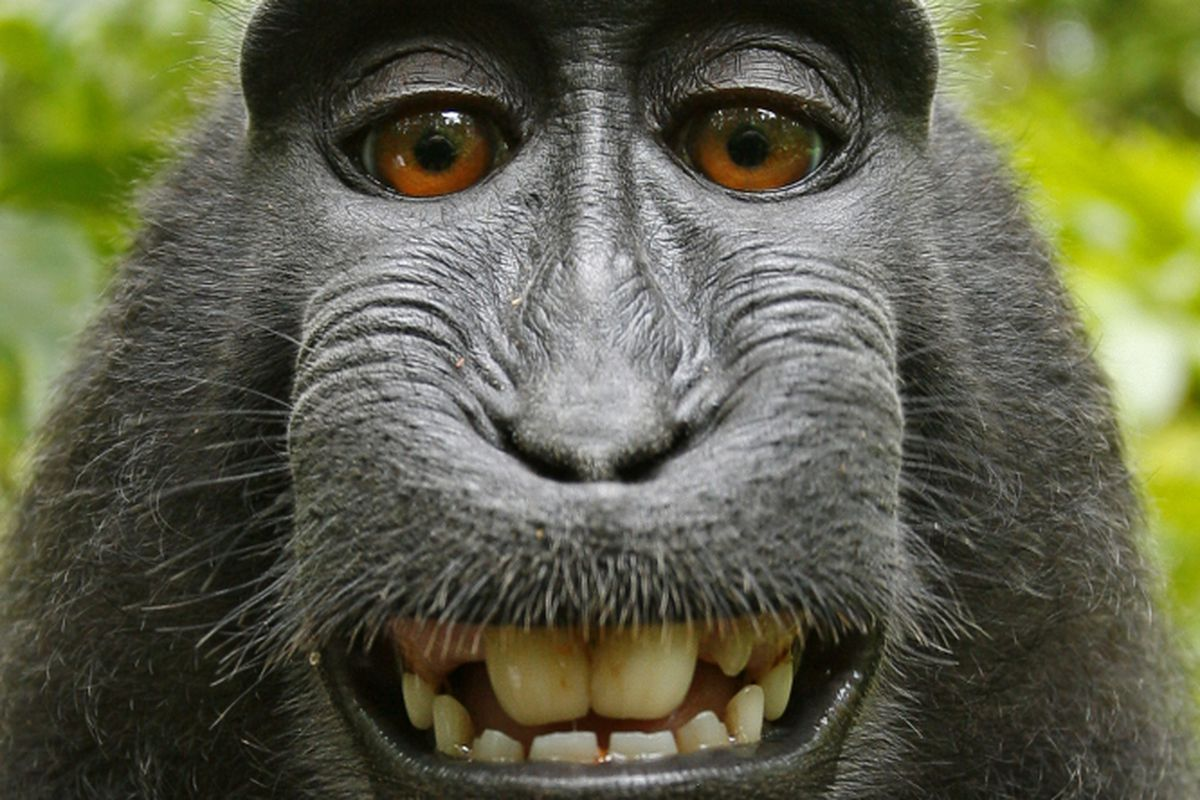
\includegraphics[width=0.7\linewidth]{animals/animal6.jpg}
    \caption{Animal 6}
    \end{minipage}
    \begin{minipage}{0.4\linewidth}
    \centering 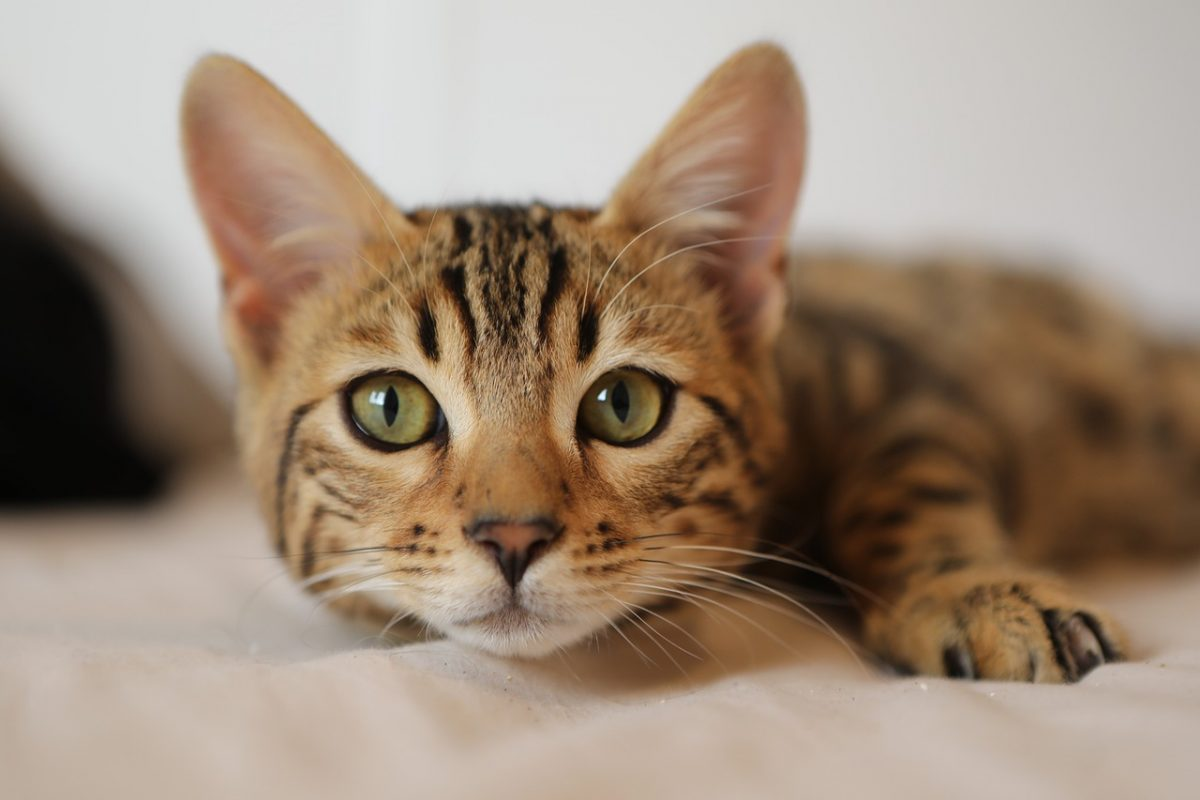
\includegraphics[width=0.7\linewidth]{animals/animal7.jpg}
    \caption{Animal 7}
    \end{minipage}
\end{figure}
\end{verbatim}
\end{scriptsize}
\vspace*{-1cm}\begin{figure}
    \centering
    \begin{minipage}{0.4\linewidth}
    \centering 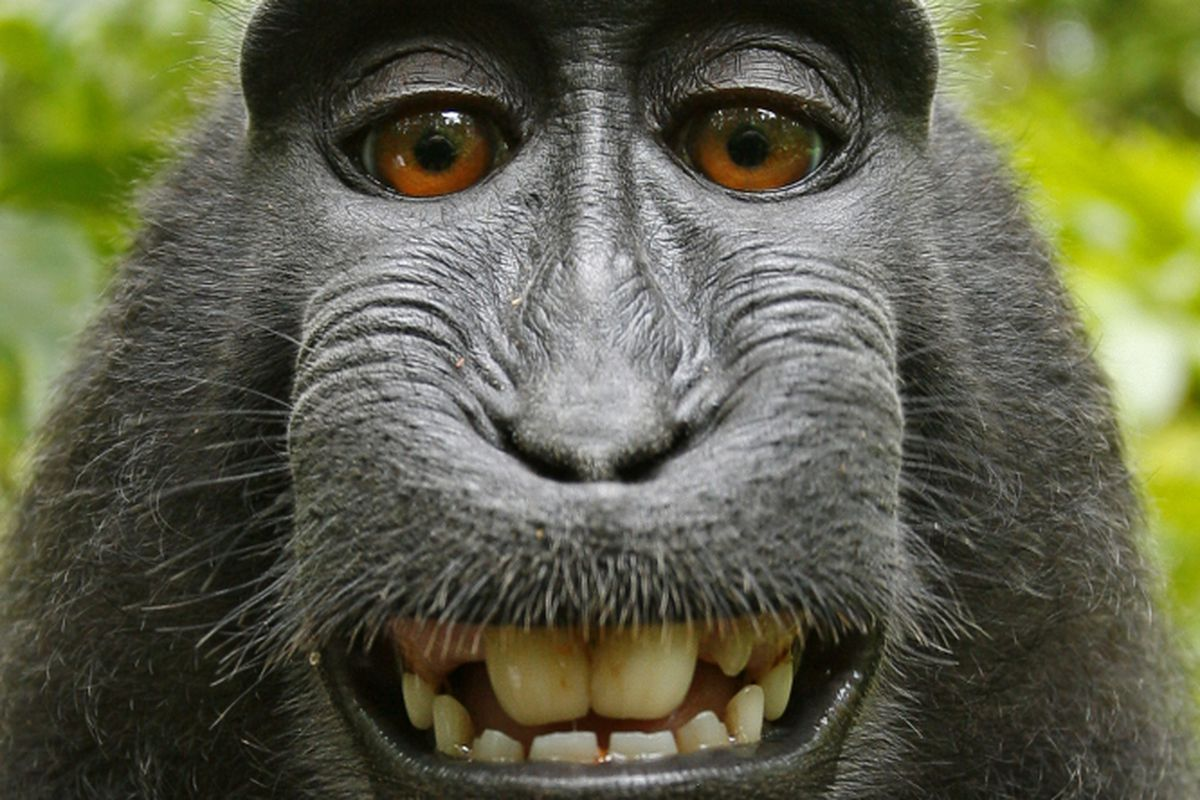
\includegraphics[width=0.7\linewidth]{animals/animal6.jpg}
    \caption{Animal 6}
    \end{minipage}
    \begin{minipage}{0.4\linewidth}
    \centering 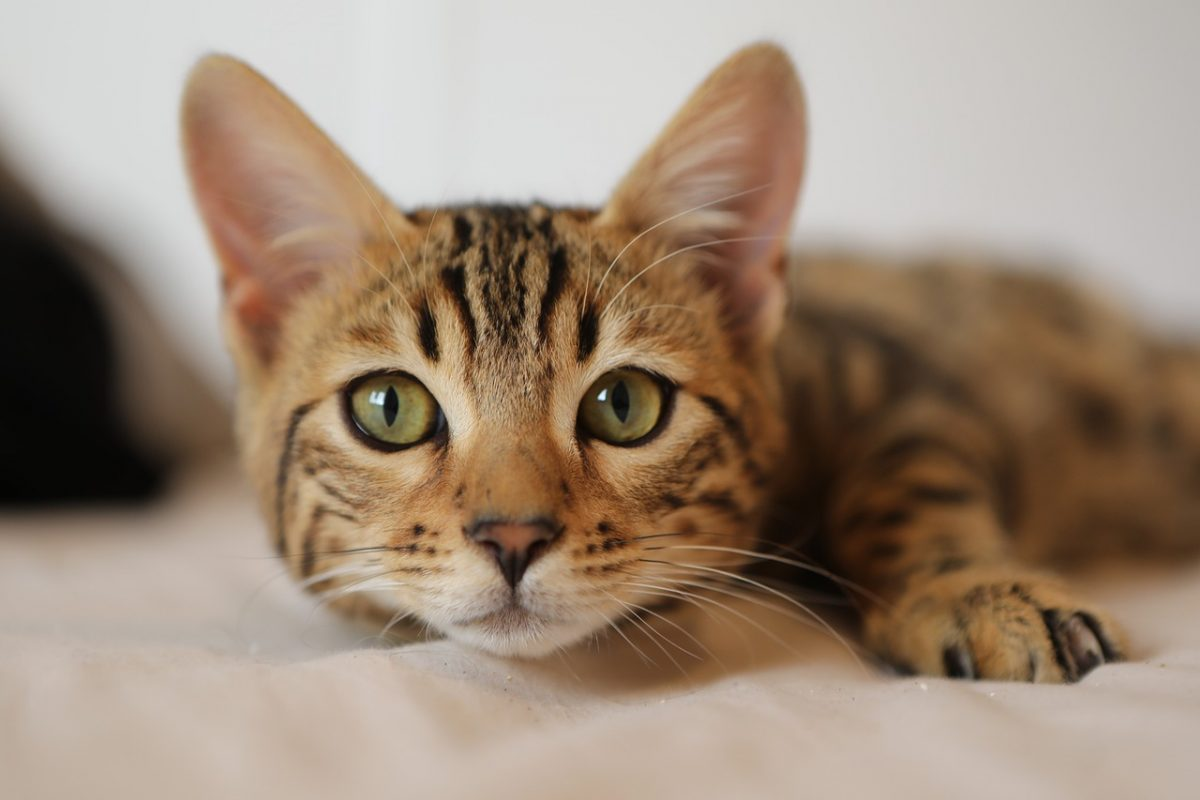
\includegraphics[width=0.7\linewidth]{animals/animal7.jpg}
    \caption{Animal 7}
    \end{minipage}
\end{figure}
\end{frame}

\begin{frame}[fragile]{Sub-imágenes: \itshape subcaption.}
\begin{scriptsize}
\begin{verbatim}
\begin{figure}
    \centering
    \begin{subfigure}{0.4\linewidth}
    \centering 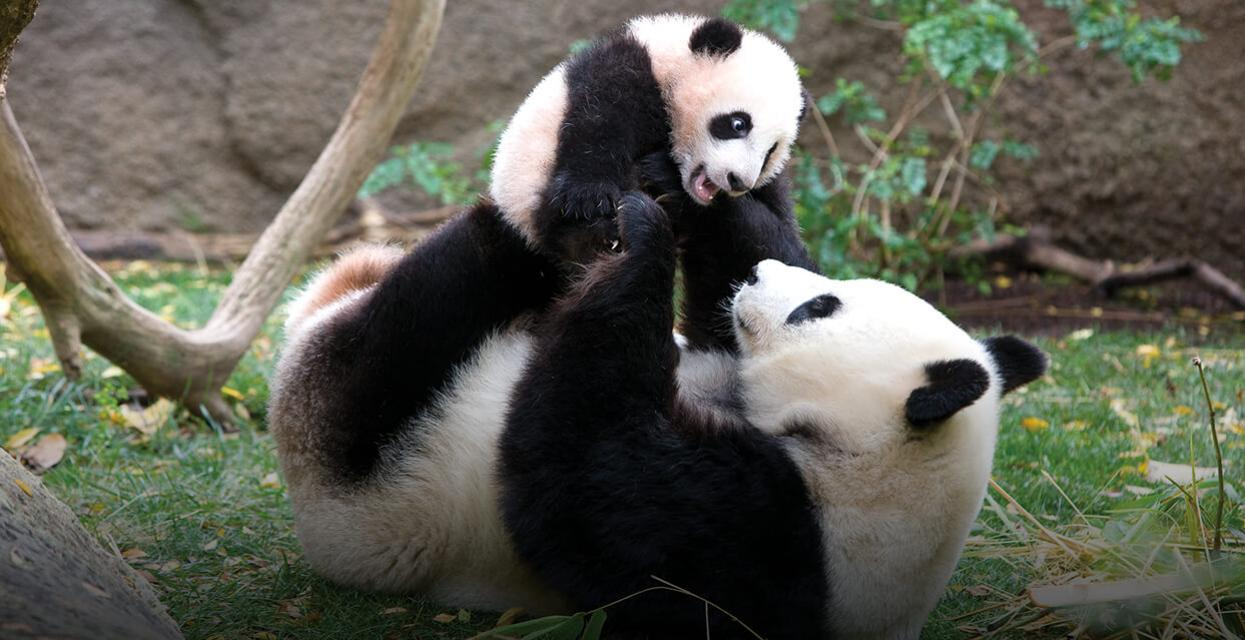
\includegraphics[width=0.7\linewidth]{animals/animal8.jpg}
    \caption{Animal 8}
    \end{subfigure}
    \begin{subfigure}{0.4\linewidth}
    \centering 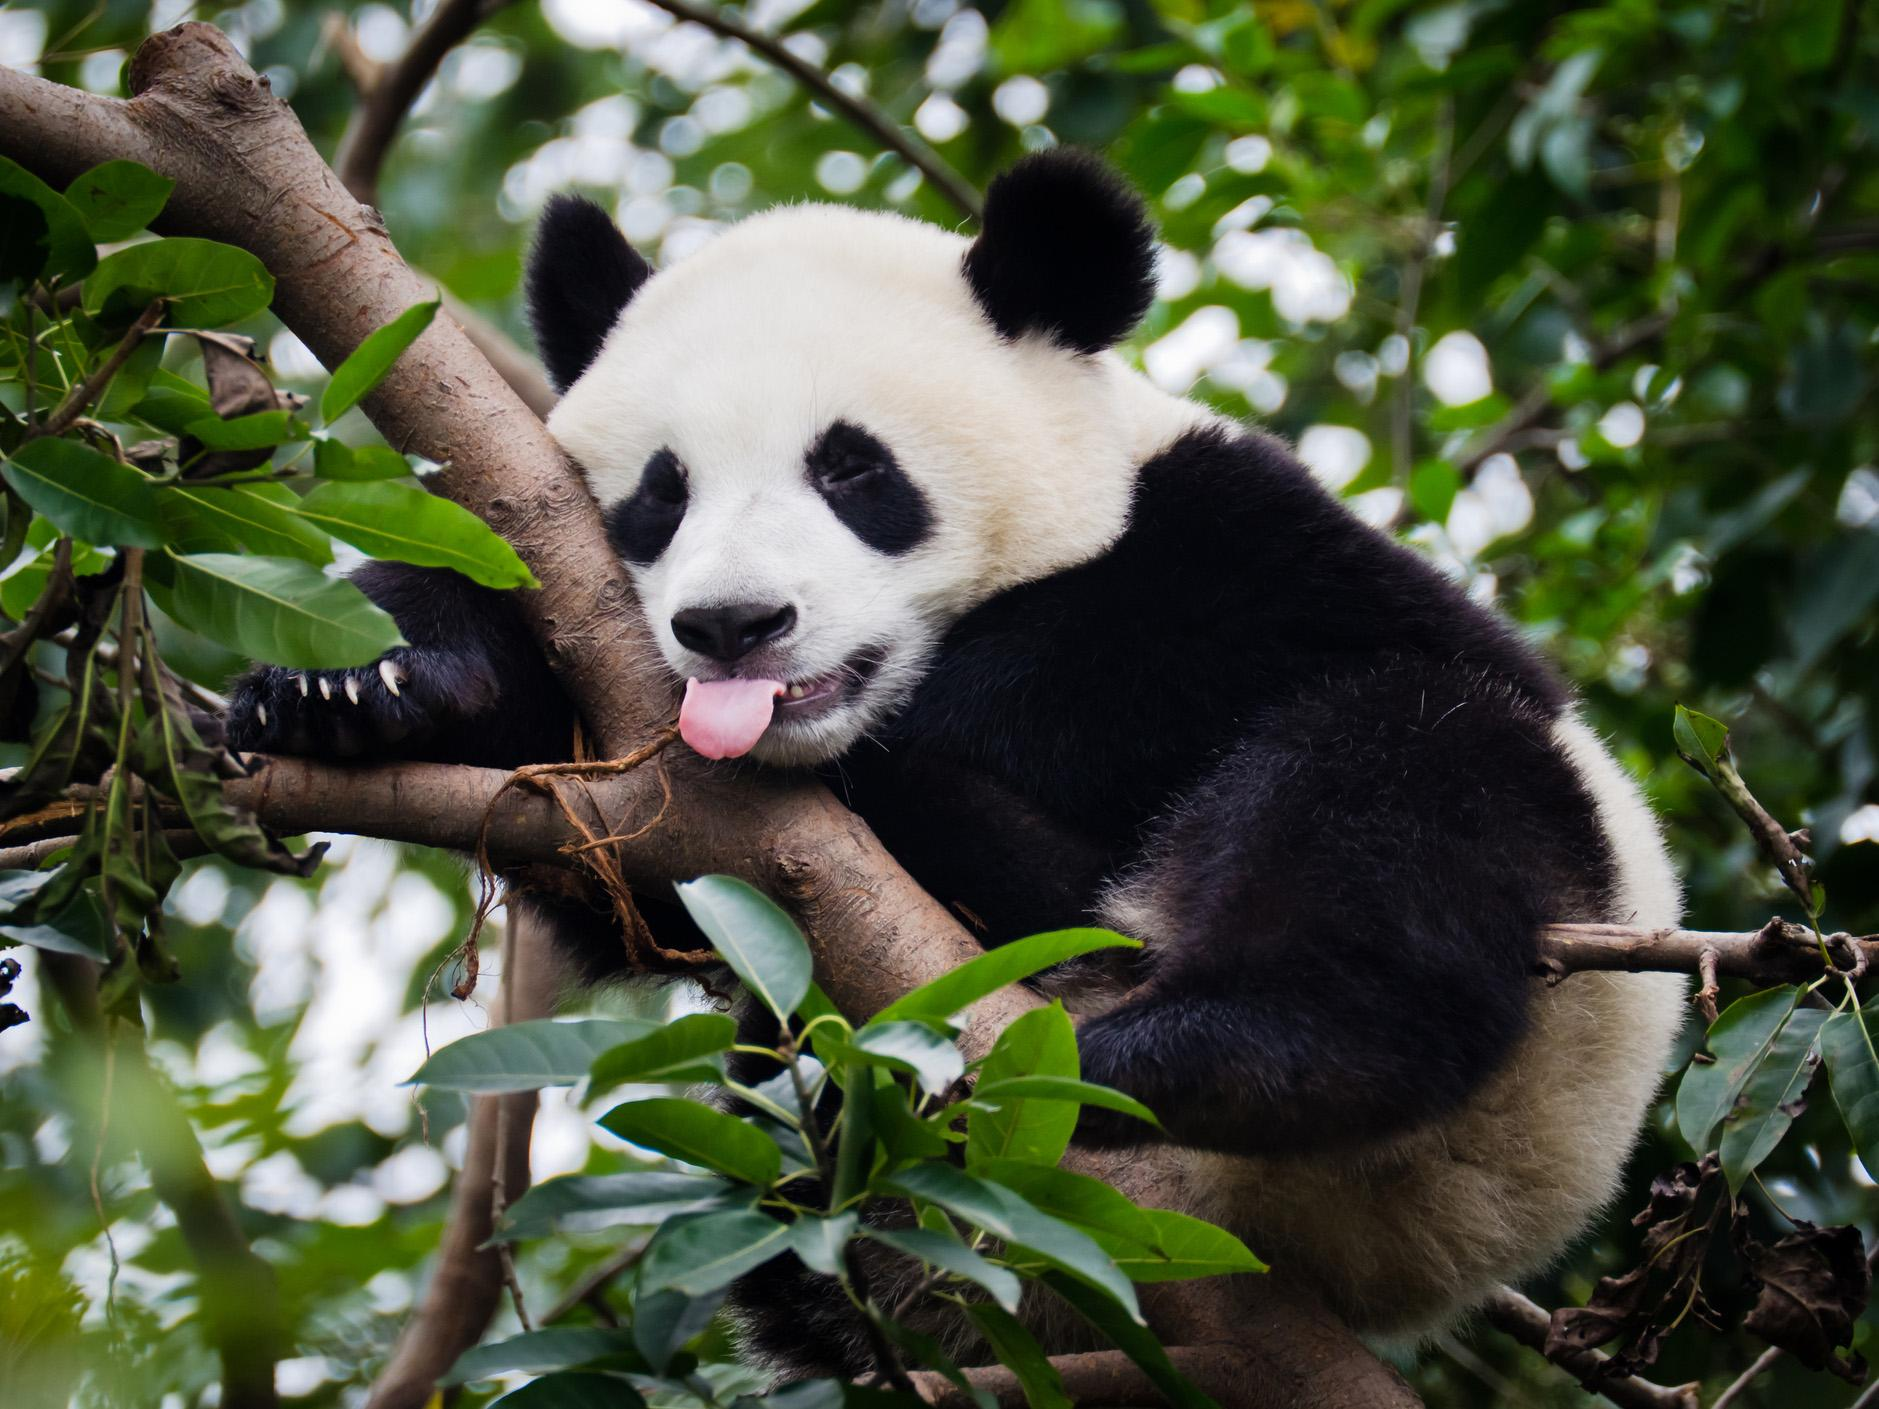
\includegraphics[width=0.7\linewidth]{animals/animal9.jpg}
    \caption{Animal 9}
    \end{subfigure}
    \caption{Imágenes de osos panda.}
\end{figure}
\end{verbatim}
\end{scriptsize}
\vspace*{-1cm}\begin{figure}
    \centering
    \begin{subfigure}{0.4\linewidth}
    \centering 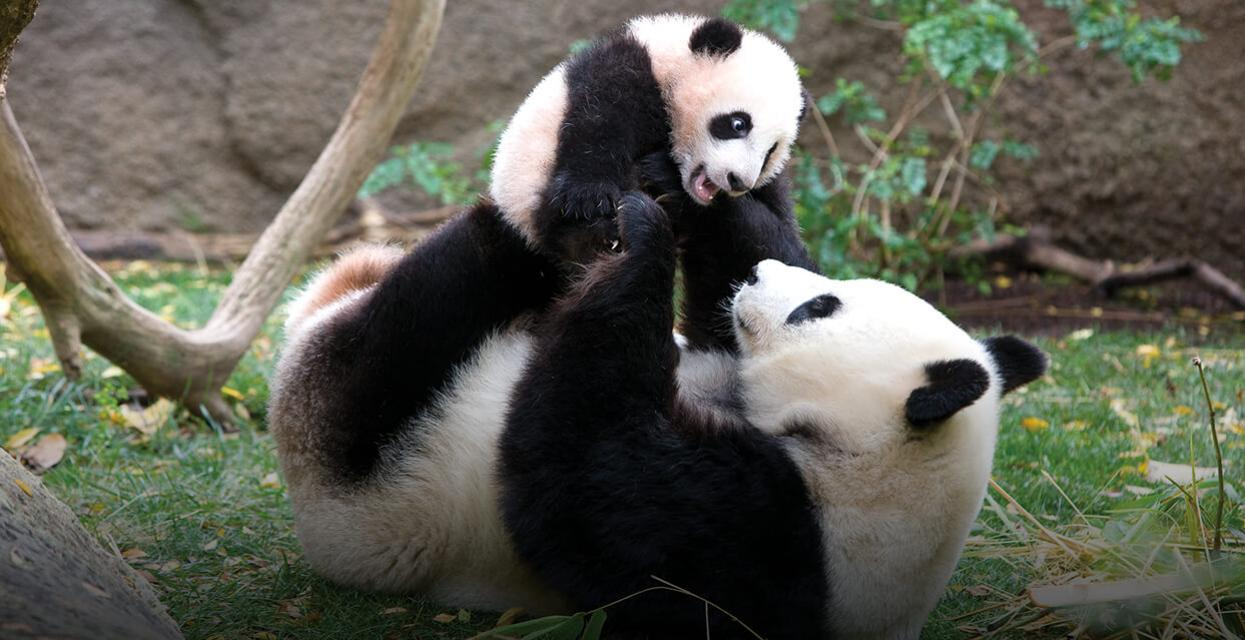
\includegraphics[width=0.7\linewidth]{animals/animal8.jpg}
    \caption{Animal 8}
    \end{subfigure}
    \begin{subfigure}{0.4\linewidth}
    \centering 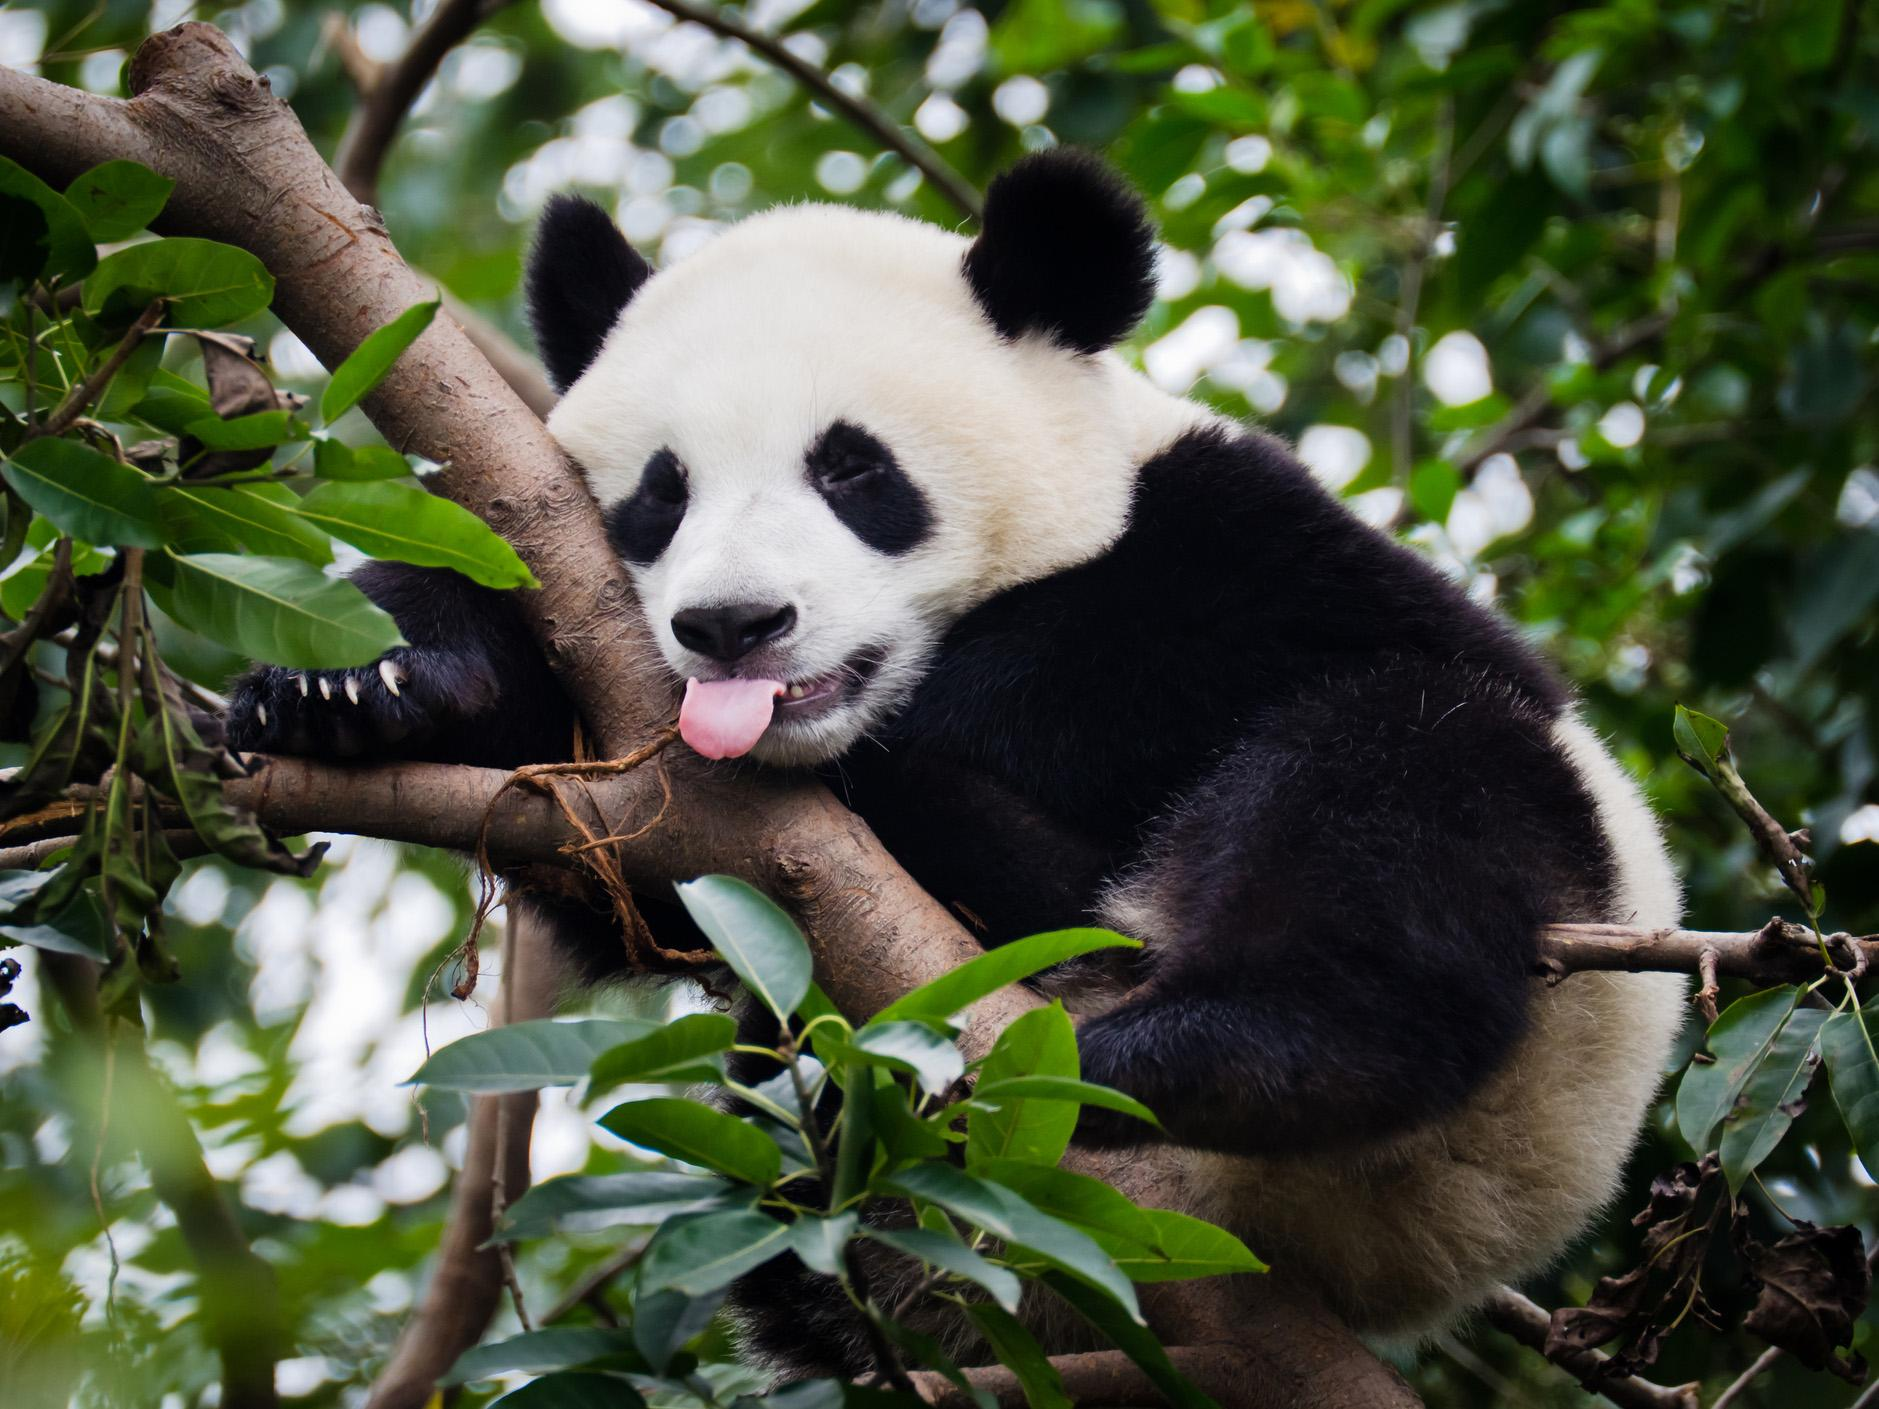
\includegraphics[width=0.7\linewidth]{animals/animal9.jpg}
    \caption{Animal 9}
    \end{subfigure}
    \caption{Imágenes de osos panda.}
\end{figure}
\end{frame}

\section{Colores.}
\begin{frame}{Contenido.}
  \tableofcontents[currentsection]
\end{frame}

\begin{frame}[fragile]{Colores.}
    Para usar colores hay que importar el paquete \verb!xcolor!\footnote{La documentación del paquete \verb~xcolor~ la pueden encontrar en \href{http://mirrors.ucr.ac.cr/CTAN/macros/latex/contrib/xcolor/xcolor.pdf}{\textcolor{colorClase}{este link}}.}.
    
    Algunos colores tienen nombre de acuerdo a la paleta que se llame en las opciones del paquete. 
    \begin{itemize}
        \item \verb!base!
        \item \verb!dvipsnames! - 68 cmyk - ideales para imprimir.
        \item \verb!svgnames! - 151 rgb - ideales para pantallas.
        \item \verb!x11names! - 317 rgb - ideales para pantallas.
    \end{itemize}
\end{frame}

\begin{frame}[fragile]{Definición de colores.}
    Se pueden definir colores en las siguientes escalas:
    \begin{itemize}
        \item core models: rgb, cmy, cmyk, hsb, gray (entre 0 y 1)
        \item integer models: RGB, HTML, HSB, Gray (depende de la escala)
        \item decimal models: Hsb, tHsb, wave (otros)
    \end{itemize}

\end{frame}
\begin{frame}[fragile]{Definición de colores.}
    \definecolor{rosado1}{rgb}{0.858, 0.188, 0.478}
    \definecolor{rosado2}{RGB}{219, 48, 122}
    \definecolor{rosado3}{cmyk}{0, 0.7808, 0.4429, 0.1412}
    \definecolor{gris1}{gray}{0.6}
    \begin{small}
    \begin{itemize}
        \item \verb!\definecolor{rosado1}{rgb}{0.858, 0.188, 0.478}!  {\color{rosado1}\rule{\linewidth}{1mm}}
        
        \item \verb!\definecolor{rosado2}{RGB}{219, 48, 122}!
        {\color{rosado2}\rule{\linewidth}{1mm}}
        \item \verb!\definecolor{rosado3}{cmyk}{0, 0.7808, 0.4429, 0.1412}!
        {\color{rosado3}\rule{\linewidth}{1mm}}
        \item \verb!\definecolor{gris1}{gray}{0.6}!
        {\color{gris1}\rule{\linewidth}{1mm}}
    \end{itemize}
\end{small}
\end{frame}

\begin{frame}[fragile]{Mezcla de colores.}
\colorlet{ModRubineRed}{RubineRed!70!}
\colorlet{color1}{green!70!orange!70!}
    Se pueden mezclar colores de la siguiente manera:
    
    \begin{itemize}
        \item \verb~\colorlet{ModRubineRed}{RubineRed!70!}~
        \item \verb~\colorlet{color1}{green!50!orange!40!}~
    \end{itemize}
    
    {\color{RubineRed} \rule{\linewidth}{1mm} }
    {\color{ModRubineRed} \rule{\linewidth}{1mm} }
    {\color{green!70} \rule{\linewidth}{1mm} }
    {\color{orange!70} \rule{\linewidth}{1mm} }
    {\color{color1} \rule{\linewidth}{1mm} }
\end{frame}

\section{Tikz.}
\begin{frame}{Contenido.}
  \tableofcontents[currentsection]
\end{frame}
\begin{frame}[fragile]{Tikz.}
    Para usar \verb!Tikz!\footnote{Para mayor información, la documentación la encuentran en \href{https://www.bu.edu/math/files/2013/08/tikzpgfmanual.pdf}{\textcolor{colorClase}{este link}}.} hay que importar los siguientes paquetes en el preámbulo:
    
    \begin{footnotesize}
    \begin{itemize}
        \item \verb!\usepackage{tikz}!
        \item \verb!\usetikzlibrary{decorations.pathmorphing, patterns,shapes}!
        \item \verb!\usetikzlibrary{positioning}!
        \item \verb!\usepackage{pgfplots}!
        \item \verb!\pgfplotsset{compat=1.12}!
    \end{itemize}
    \end{footnotesize}
    
    
\end{frame}

\subsection{Tikzpicture.}
\begin{frame}{Contenido.}
  \tableofcontents[currentsubsection]
\end{frame}

\begin{frame}[fragile]{Tikzpicture: nodos y caminos.}
\begin{minipage}{0.4\linewidth}
\begin{tiny}
\begin{verbatim}
\begin{figure}
\centering
\begin{tikzpicture}
\node[fill=Seashell4!80, draw=white, circle](A) {A};
\node[fill= LightGoldenrod1,  ellipse] (B) [above right = 1cm and 1.5cm of A] {B};
\node[fill= Tomato1, draw=black, ellipse] (C) [below right = 0.6cm and 2cm of A] {C};

\path[every node/.style={font=\sffamily\small}]
(A) edge (B)
edge[-, very thick] (C)
(B) edge[dashed] (C)
edge[->, thick, dashed, bend right] (A)
(C) edge[<->, thick, bend left] (A);
\end{tikzpicture}
\end{figure}
\end{verbatim}
\end{tiny}
\end{minipage}
\begin{minipage}{0.4\linewidth}
\vspace*{4cm}
\begin{figure}
\centering
\begin{tikzpicture}
\node[fill=Seashell4!80, circle](A) {A};
\node[fill= LightGoldenrod1, ellipse] (B) [above right = 1cm and 1.5cm of A] {B};
\node[fill= Tomato1, ellipse] (C) [below right = 0.6cm and 2cm of A] {C};

\path[every node/.style={font=\sffamily\small}]
(A) edge (B)
edge[-, very thick] (C)
(B) edge[dashed] (C)
edge[->, thick, dashed, bend right] (A)
(C) edge[<->, thick, bend left] (A);
\end{tikzpicture}
\end{figure}
\end{minipage}
\end{frame}

\subsection{Circulares.}
\begin{frame}{Contenido.}
  \tableofcontents[currentsubsection]
\end{frame}

\begin{frame}[fragile]{Circulares.}
    Para hacer diagramas circulares (pie) hay que poner en el preámbulo\footnote{En overleaf no está funcionando este paquete entonces hay que poner el .sty en su carpeta. La documentación la encuentran en \href{http://mirrors.ucr.ac.cr/CTAN/graphics/pgf/contrib/pgf-pie/pgf-pie-manual.pdf}{\textcolor{colorClase}{este link}}.}
    
    \verb!\usepackage{pgf-pie}!
    
    
\end{frame}

\begin{frame}[fragile]{Circulares.}
\begin{figure}
\begin{minipage}{0.4\linewidth}
\hspace*{-3cm}\begin{scriptsize}
\begin{verbatim}
\begin{tikzpicture}
\pie
{24/A,25/B, 46/C,2/D, 2/E,1/F}
\end{tikzpicture}
\end{verbatim}
\end{scriptsize}
\end{minipage}
\begin{minipage}{0.4\linewidth}
\centering
\scalebox{0.6}{
\begin{tikzpicture}
\pie
{24/A,25/B, 46/C,2/D, 2/E,1/F}
\end{tikzpicture}
}
\end{minipage}
    \end{figure}
\end{frame}

\begin{frame}[fragile]{Circulares: polares.}
\begin{figure}
\begin{minipage}{0.4\linewidth}
\hspace*{-3cm}\begin{scriptsize}
\begin{verbatim}
\begin{tikzpicture}
\pie[polar, text=pin, rotate=45]
{24/A,25/B, 46/C,2/D, 2/E,1/F}
\end{tikzpicture}
\end{verbatim}
\end{scriptsize}
\end{minipage}
\begin{minipage}{0.4\linewidth}
\centering
\scalebox{0.6}{
\begin{tikzpicture}
\pie[polar, text=pin, rotate=45]
{24/A,25/B, 46/C,2/D, 2/E,1/F}
\end{tikzpicture}
}
\end{minipage}
    \end{figure}
\end{frame}

\begin{frame}[fragile]{Circulares: cuadrados.}
\begin{figure}
\begin{minipage}{0.4\linewidth}
\hspace*{-3cm}\begin{scriptsize}
\begin{verbatim}
\begin{tikzpicture}
\pie[square, text=inside,
scale font]
{24/A,25/B, 46/C,2/D, 2/E,1/F}
\end{tikzpicture}
\end{verbatim}
\end{scriptsize}
\end{minipage}
\begin{minipage}{0.4\linewidth}
\centering
\scalebox{0.6}{
\begin{tikzpicture}
\pie[square, text=inside,
scale font]
{24/A,25/B, 46/C,2/D, 2/E,1/F}
\end{tikzpicture}
}
\end{minipage}
    \end{figure}
\end{frame}

\begin{frame}[fragile]{Circulares: nubes.}
\begin{figure}
\begin{minipage}{0.4\linewidth}
\hspace*{-5cm}\begin{scriptsize}
\begin{verbatim}
\begin{tikzpicture}
\pie[cloud, text=legend,
scale font]
{24/A,25/B, 46/C,2/D, 2/E,1/F}
\end{tikzpicture}
\end{verbatim}
\end{scriptsize}
\end{minipage}
\begin{minipage}{0.4\linewidth}
\centering
\scalebox{0.6}{
\begin{tikzpicture}
\pie[cloud, text=legend, scale font]
{24/A,25/B, 46/C,2/D, 2/E,1/F}
\end{tikzpicture}
}
\end{minipage}
    \end{figure}
\end{frame}


\section{Actividad} 
\begin{frame}{Contenido.}
  \tableofcontents[currentsection]
\end{frame}
\begin{frame}[fragile]{Ejercicio. (Actividad 5: nombre.tex y nombre.pdf)}
En un documento \verb!article! desarrolle lo siguiente:
\begin{scriptsize}
\begin{multicols}{2}
\begin{enumerate}
    \item Cree lineas de los siguientes colores:
    \begin{itemize}
        \item Magenta4
        \item 60\% Seashell4 y 100\% SlateBlue4
        \item 20\% blue y 40\% red
        \item Tomato1
        \item Firebrick1
        \item 50\% Firebrick4 y 90\% DeepPink1
        \item rgb 0.169,0, 0.6 
    \end{itemize}
    Para crear una linea: \verb!{\color{color}\rule{ancho}{alto}}!
    \item Inserte todas las imágenes de la carpeta como subfigures (que todas quepan en una página)
    \item Cree un \verb!Tikz! de nodos y caminos con las siguientes especificaciones:
    \begin{itemize}
        \item 5 nodos: A, B, ... , E.
        \item A está en el centro.
        \item Todos los nodos están conectados a A en linea punteada (excepto B) recta.
        \item B y C están conectados con línea punteada y curva. 
    \end{itemize}
    \item Cree un \verb!Tikz! circular de nubes con A:10\%, B:23\%, C:5\%, D:10\%, E:12\%, F:17\%, G:20\%, H:3\%. El texto pineado y ajustado al tamaño. 
\end{enumerate}
\end{multicols}
\end{scriptsize}
\end{frame}
{
% all template changes are local to this group.
    \setbeamertemplate{navigation symbols}{}
    \setbeamercolor{background canvas}{bg=colorClase}
    \begin{frame}[plain, noframenumbering]
    \vfill
    \begin{center}
    \begin{Huge}
        %\textcolor{white}{Gracias!}
    \end{Huge}
    \end{center}
    \vfill
     \end{frame}
}
            
\end{document}